%&pdfLaTeX
% !TEX encoding = UTF-8 Unicode
\documentclass[a4paper]{article}

\usepackage{datetime}
\usepackage{ifxetex}
\ifxetex
\usepackage{fontspec}
\setmainfont[Mapping=tex-text]{STIXGeneral}
\else
\usepackage[T1]{fontenc}
\usepackage[utf8]{inputenc}
\fi

\usepackage{textcomp}
\usepackage{graphicx}
\graphicspath{{figures/}{ordalie_documentation/}}
\usepackage{array}
\usepackage{amssymb}
\usepackage{fancyhdr}
\usepackage{verbatim}
\usepackage{textgreek}

%%\usepackage[backend=biber]{biblatex}
%%\addbibresource{softbib}
\usepackage{url}


\renewcommand{\headrulewidth}{0pt}
\renewcommand{\footrulewidth}{0pt}

\newcommand{\specialcell}[2][l]{%
  \begin{tabular}[#1]{@{}l@{}}#2\end{tabular}}


\newcommand{\paraluc}[1]{
\smallskip
  \paragraph{#1}\mbox{}\\
}

\newcommand{\idee}[1]{
  \begin{table}[h!]
    \begin{tabular}{|p{0.1\textwidth}p{0.9\textwidth}|}
      \hline
      &\hspace{1ex}\\
      \begin{tabular}{c}
\includegraphics[scale=0.2]{ampoule2.png}\end{tabular} & \begin{tabular}{p{0.8\textwidth}} #1 \end{tabular}\\
      &\hspace{1ex}\\
      \hline
    \end{tabular}
  \end{table}
}

\newcommand{\attention}[1]{
  \begin{table}[h!]
    \begin{tabular}{|p{0.1\textwidth}p{0.9\textwidth}|}
      \hline
      &\hspace{1ex}\\
      \begin{tabular}{c}
\includegraphics[scale=1.0]{attention.png}\end{tabular} & \begin{tabular}{p{0.8\textwidth}} #1 \end{tabular}\\
      &\hspace{1ex}\\
      \hline
    \end{tabular}
  \end{table}
}

%%\newcommand{\subsubsubsection}[1]{\paraluc{#1}\mbox{}\\}
\setcounter{secnumdepth}{4}
\setcounter{tocdepth}{4}



\begin{document}

%%\begin{figure}[htbp]

\includegraphics[width=\textwidth, keepaspectratio=true]{ordalie_title.jpg}
%%\caption{This should be the caption for \texttt{figures/ordalie\_documentation-fig001.jpg}.}
%%\end{figure}

\begin{center}
{\Huge\bf The manual}


Version 3.5
\end{center}

\vspace{10cm}

\begin{tabular}{l}
\copyright 1997-\the\year{}   Luc Moulinier and CSTB\\
\\
\\
Complex Systems and Translational Bioinformatics, \\
The ICube laboratory\\
Centre de Recherches Biomédicales de Strasbourg (CRBS)\\
1, rue Eugène Boeckel\\
67 000 Strasbourg\\
FRANCE\\
\end{tabular}
 
\newpage
\tableofcontents

\newpage
\section{Installing Ordalie}

\subsection{System Requirements}
Ordalie is a cross-platform application available for Windows, MacOS, and Linux (32/64-bit architectures). 

\subsubsection{Graphics}
To render 3D structures, Ordalie leverages the \textbf{OpenGL} library. While this is standard on most modern graphics cards, specific attention is needed for certain systems:

\attention{On MacOS (version \textit{Mojave} and later), OpenGL is no longer bundled with the OS by default. Users may need to install it manually (e.g., via the \textit{App Store} or developer tools) to enable 3D visualization.}

\subsubsection{Connectivity}
While Ordalie functions offline, an active internet connection is highly recommended to access remote features, including:
\begin{itemize}
    \item Direct querying of biological databases (PDB, UniProt, NCBI).
    \item On-the-fly sequence alignments.
    \item Web service integration.
\end{itemize}

\subsection{Installation Procedure}
The latest version of Ordalie can be downloaded from: \url{http://www.lbgi.fr/ordalie}. Select the installer corresponding to your platform (Windows, MacOS, or Linux 64-bit).

\subsubsection{Windows Installation}
Launch the \texttt{.exe} installer and follow the on-screen instructions. Upon completion, Ordalie will launch automatically, and a shortcut will be created on your desktop.

\subsubsection{Linux and MacOS Installation}
For Unix-based systems, Ordalie is provided as a compressed archive. Follow these steps in your terminal to complete the installation:

\begin{enumerate}
    \item \textbf{Extract the archive:} \\
    \texttt{\% tar -zxf setup-ordalie-linux-x86\_64.tar.gz}
    \item \textbf{Run the installation script:} \\
    \texttt{\% cd setup-ordalie-linux-x86\_64} \\
    \texttt{\% ./install.tcl}
\end{enumerate}

\paragraph{Directory Selection:} By default, Ordalie installs to your \texttt{/home/<user>/} directory. If you wish to install it system-wide (e.g., in \texttt{/usr/local}), ensure you have the necessary \texttt{sudo} or administrative privileges.

\paragraph{Cleanup:} Once the installation is confirmed, you may safely delete the setup directory: \\
\texttt{\% cd ..} \\
\texttt{\% rm -rf setup-ordalie-linux-x86\_64}


\newpage
\section{Introduction}

\subsection{Context}
Proteins, one of the fundamental building blocks of life, can be classified into various hierarchical categories based on their structural and functional similarities. This classification helps scientists understand protein evolution, function, and relationships. Since the 1970s, the massive increase of protein 3D structures and sequences has led to more subtle definitions, such as super-family or sub-family organizations.

\begin{itemize}
\item \textbf{Super-family:} The broadest level of classification. Members share distant evolutionary ancestry and often a common structural fold, performing a wide range of biological roles.
\item \textbf{Family:} Proteins within a super-family that are more closely related in terms of sequence, structure, and function, typically sharing a common evolutionary origin.
\item \textbf{Sub-family:} The most specific level. Members are highly related, often performing near-identical functions and having evolved recently from a common ancestor. 
\end{itemize}

This introduces a granularity in the protein family concept, providing several scales for analysis that allow for the identification of the zones or residues responsible for this functional divergence.

\subsection{Ordalie}
Ordalie (ORDered ALignment Information Explorer) is an interactive tool designed for the exploration of the informational content of a Multiple Sequence Alignment (MSA) in a hierarchical manner, and within different contexts, such as phylogeny or 3D structure.

\begin{figure}[htbp]
\centering
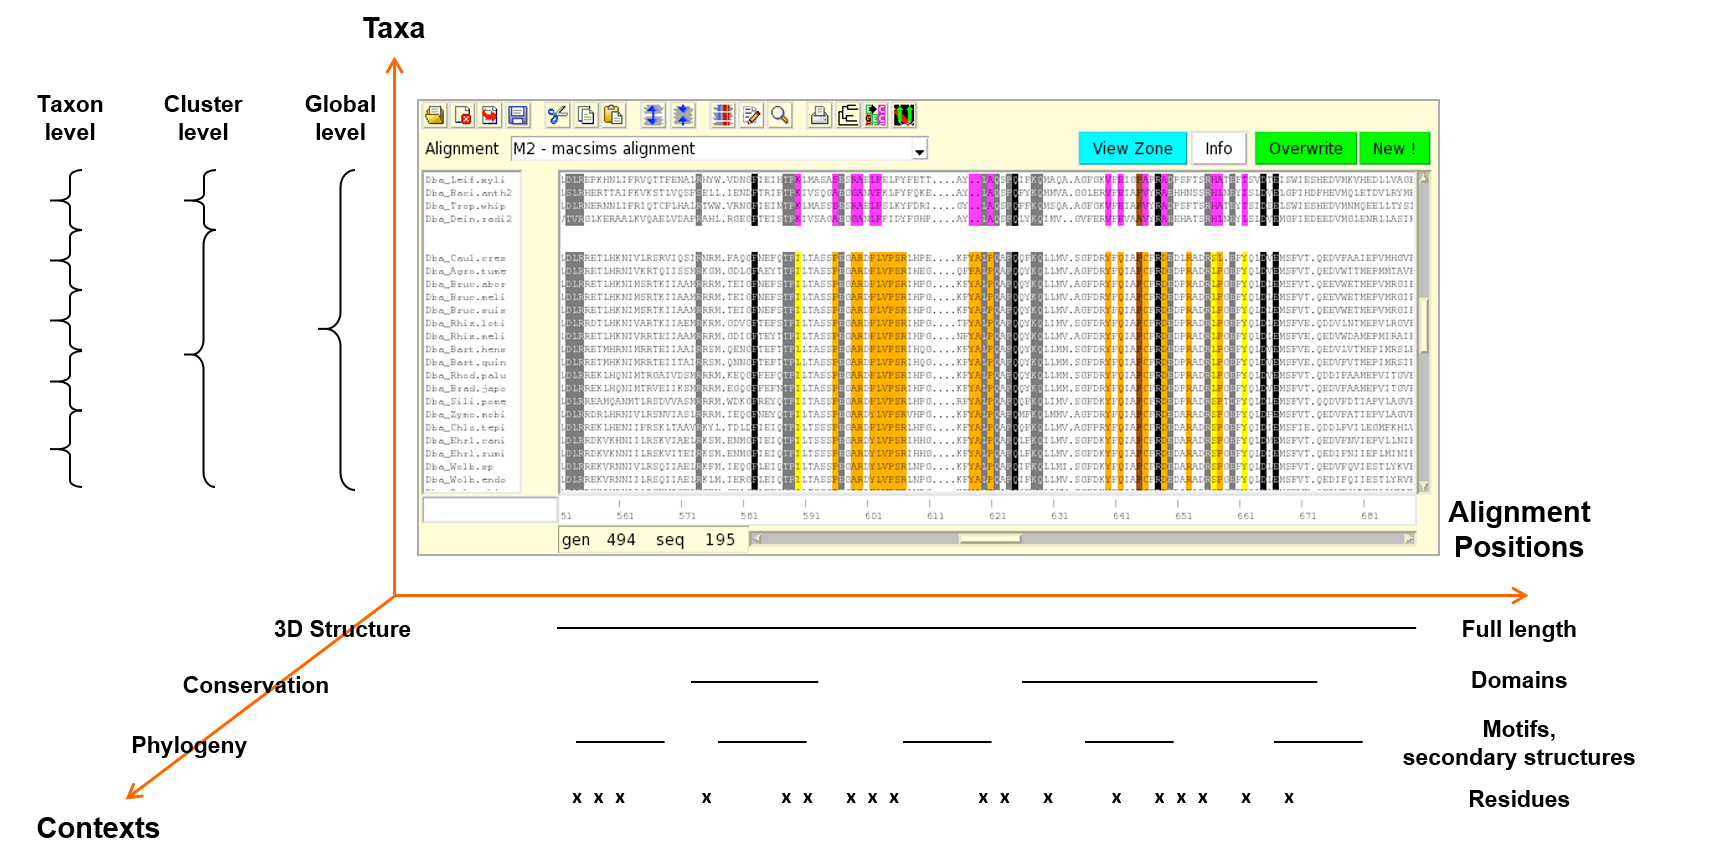
\includegraphics[width=\textwidth, keepaspectratio=true]{ordalie_philosophy.png}
\caption{Diagram of the Ordalie philosophy}
\label{ordaliephilo}
\end{figure}

The Ordalie philosophy (see fig. \ref{ordaliephilo}) resides in its capacity to perform a concomitant multi-scale analysis across three axes: the amino acid sequence axis, the taxa axis, and the contexts axis.

The information distributed along the sequence (horizontal axis) is analyzed across several scales:
\begin{itemize}
    \item \textbf{Large-scale features:} e.g. Overall domain architecture and broad evolutionary conserved regions.
    \item \textbf{Intermediate-scale features:} e.g. Secondary structure elements, functional motifs (SLiMs), and molecular recognition patches.
    \item \textbf{Local features:} e.g. Post-translational modification (PTM) sites, catalytic residues, and site-specific conservation scores.
\end{itemize}

The taxonomic depth constitutes the second axis:
\begin{itemize}
\item \textbf{Global scale:} To define family-wide hallmarks and conserved motifs.
\item \textbf{Intermediate scale:} To distinguish sub-families by identifying residues specifically conserved within a subgroup.
\item \textbf{Individual scale:} To pinpoint mutations or unique variations specific to a particular taxon.
\end{itemize} 

The third analytical axis focuses on computational contexts, unified within a structural framework. This allows sequence-based features to be spatially mapped and compared directly onto 3D structures.

\subsection{Database and Instance Management}
\label{intro-db-instance}

At the core of Ordalie lies a dedicated \textbf{SQLite database} engine. This architecture ensures high-performance data handling and persistent storage for both system-wide configurations and alignment-specific data.

A major strength of this architecture is the ability to perform non-linear, exploratory analyses through a system of \textbf{Instances}. Rather than a linear versioning system, instances in Ordalie represent parallel analytical hypotheses. They allow the user to freeze and compare different interpretations of the same dataset:

\begin{description}
    \item[The Database:] Acts as a central, relational repository. By using the native \texttt{.ord} file format, all sequences, metadata, and analytical branches are bundled into a single, portable file, ensuring data integrity across sessions.
    \item[Instances:] An \textit{instance} captures a specific state of the exploratory process. It is not merely a backup, but a record of a particular scientific choice, such as:
    \begin{itemize}
        \item A specific \textbf{clustering strategy} (e.g., comparing different phylogenetic groupings or functional sub-families).
        \item A unique \textbf{alignment topology}: This allows for the comparison of different ways to register sequence zones. For example, a specific domain can be anchored to one position in one instance and realigned to a different evolutionary landmark in another.
        \item A unique set of curated \textbf{sequence features} or annotations mapped onto a given alignment solution.
    \end{itemize}
\end{description}

Instances are managed via the dedicated \textit{Instance Bar} (see section \ref{instance-bar}), providing a seamless way to switch between different analytical scenarios without data loss.

\newpage
\section{Ordalie Basics}
This section presents the fundamental operations and interface logic of Ordalie. While these concepts are introduced here, they are explored in greater detail in the specialized sections of this manual.

\subsection{Alignment Handling}
Ordalie supports a wide range of MSAs file formats, including FASTA, MSF, RSF, ClustalW ALN, Macsim/XML, and its native ORD format. The file format is chosen in the \texttt{File} $\rightarrow$ \texttt{Open ...} sub-menu. When a file is given on the command line, its format is deduced from its extension; if the extension is unknown, Ordalie tries to detect the format from the file content and, failing that, asks the user. Only one alignment can be opened at a time: use \texttt{File} $\rightarrow$ \texttt{Close} before opening another one.
\smallskip
Basic statistical information is automatically logged in the \textit{Log Console} for both the global alignment and individual sequences (e.g., length, isoelectric point). Pairwise identity scores are also computed and logged for the global set and any defined groups.

\subsection{Instances}
As already mentioned in the introduction (see \ref{intro-db-instance}) a single Multiple Sequence Alignment can be the subject of various analytical interpretations. In Ordalie, these distinct states—such as different clustering configurations or specific conservation models—are called \textbf{Instances}. This system allows users to explore multiple hypotheses in parallel, with the ability to annotate, save, and switch between states without data loss (see \ref{instance-bar}). This non-linear workflow is made possible by the integrated SQLite database.
\smallskip
The first instance, named \textit{Original alignment}, is a read-only copy of the loaded alignment: it cannot be overwritten, and any modification of it must be saved as a new instance.

\subsection{Sequence Names and Databases}
Ordalie automatically parses sequence names to identify UniProt, RefSeq, or PDB accessions. By default, common database prefixes (e.g.\ \texttt{sw|} or \texttt{sp|} for SwissProt, \texttt{tr|} for TrEMBL, \texttt{ref|} for RefSeq) are stripped for clarity; for example, \texttt{>sw|P12345} is displayed as \texttt{P12345}. Prefixes are recognized whatever their case, followed either by \texttt{|} or by \texttt{:}. The \texttt{lcl|} prefix is always removed, while the \texttt{PDB} prefix is always kept since it is used to identify 3D structures. Prefix removal can be switched off, and prefixes can be added or removed, in \textit{Preferences} (see figure~\ref{preferences}).
\smallskip
If sequence names follow standard accession formats, Ordalie can fetch additional metadata from remote databases (see \ref{tool-inforetrieve}).
\smallskip
\textit{Note: While DNA/RNA alignments can be viewed or edited, Ordalie is primarily optimized for protein sequences; some advanced analytical tools may be disabled for nucleotide data.}

\subsection{Conventions and Selections}

\subsubsection{Mouse and Keyboard terminology}
In this manual, the mouse buttons are designated as \textbf{<B1>} (Left), \textbf{<B2>} (Middle), and \textbf{<B3>} (Right). Keyboard keys are represented between brackets (e.g., \texttt{<Ctrl>}).

\subsubsection{Selection Mechanisms}
Ordalie uses a standardized selection logic for both sequence names and residue ranges.

\paragraph{Sequence Names Selection}

Sequence names selection is done using a combination of <B1>, <Shift> and <Control> keys, in the same way as in most programs.
\begin{table}[h!]
\centering
\begin{tabular}{|l|p{10cm}|}
\hline
\textbf{Action} & \textbf{Result} \\
\hline
\hline
\texttt{<B1>} & Selects the sequence under the pointer. \\
\hline
\texttt{<Ctrl> + <B1>} & \textbf{Toggle selection:} Adds an unselected sequence to the current selection or removes a selected one. \\
\hline
\texttt{<Shift> + <B1>} & \textbf{Range selection:} Selects all sequences between the previous selection and the current click. \\
\hline
\texttt{<Ctrl> + <a>} & Selects all sequences in the instance. \\
\hline
\texttt{<Ctrl> + <x>} / \texttt{<c>} / \texttt{<v>} & Cut / Copy / Paste the selected sequences (same as the \texttt{Edit} menu). \\
\hline
\end{tabular}
\caption{Shortcuts for sequence name manipulation.}
\end{table}

\textit{Note: these keyboard shortcuts act when the mouse pointer is over the sequence names pane.}

\attention{If a sequence is duplicated using \texttt{Copy} then \texttt{Paste}, its name will be suffixed by \emph{\_\_<n>} where \emph{n} is the copy number.}

\paragraph{Residue Range Selection}
By default, residue range selection is disabled in Ordalie. It is enabled within specific modules (Cluster, Tree, Identity, etc.).
\begin{table}[h]
\centering
\begin{tabular}{|l|p{10cm}|}
\hline
\textbf{Action} & \textbf{Result} \\
\hline
\hline
\texttt{<B1>} & Sets the start of the selection zone. \\
\hline
\texttt{<B3>} & Sets the end of the selection zone (highlighted in grey). \\
\hline
\texttt{<Ctrl> + <B3>} & Unselects the zone under the mouse pointer. \\
\hline
\texttt{<Ctrl> + <B1>} & Selects the columns of the \textbf{feature item} (e.g., a PFAM domain) under the pointer. The feature must be displayed (\textbf{Feature} combobox of the tool). \\
\hline
\end{tabular}
\caption{Shortcuts for residue and feature selection.}
\end{table}

Several zones can be defined one after the other, either by left/right clicks and/or feature item selection. To select a feature item, first display the feature with the \textbf{Feature} combobox of the tool, then click on the item with \texttt{<Ctrl> + <B1>}.

\subsection{The SQLite Database and .ord Format}
Ordalie uses an embedded SQLite database to manage complex data structures (system data, instances, features). The \textbf{.ord} file is a compressed archive (\texttt{tar.gz}) of serialized SQLite databases:
\begin{itemize}
    \item the main database: session state (settings, trees, overview windows), sequence metadata (pI, descriptions, taxonomy...), all instances with their clusterings, features, conservation scores and annotations;
    \item one database per 3D structure (atoms, residues, chains and the 3D objects defined in the viewer), so that structures and superpositions are restored without downloading them again.
\end{itemize}
Using the \texttt{.ord} format as your primary working file is highly recommended to ensure all analytical context is preserved.
\smallskip
The scheme of the database can be found in Appendix \ref{chap-schemedb}.


\subsection{The Main Window}
The interface is organized vertically into several functional areas (see fig. \ref{mainwindow}).

\begin{figure}[htbp]
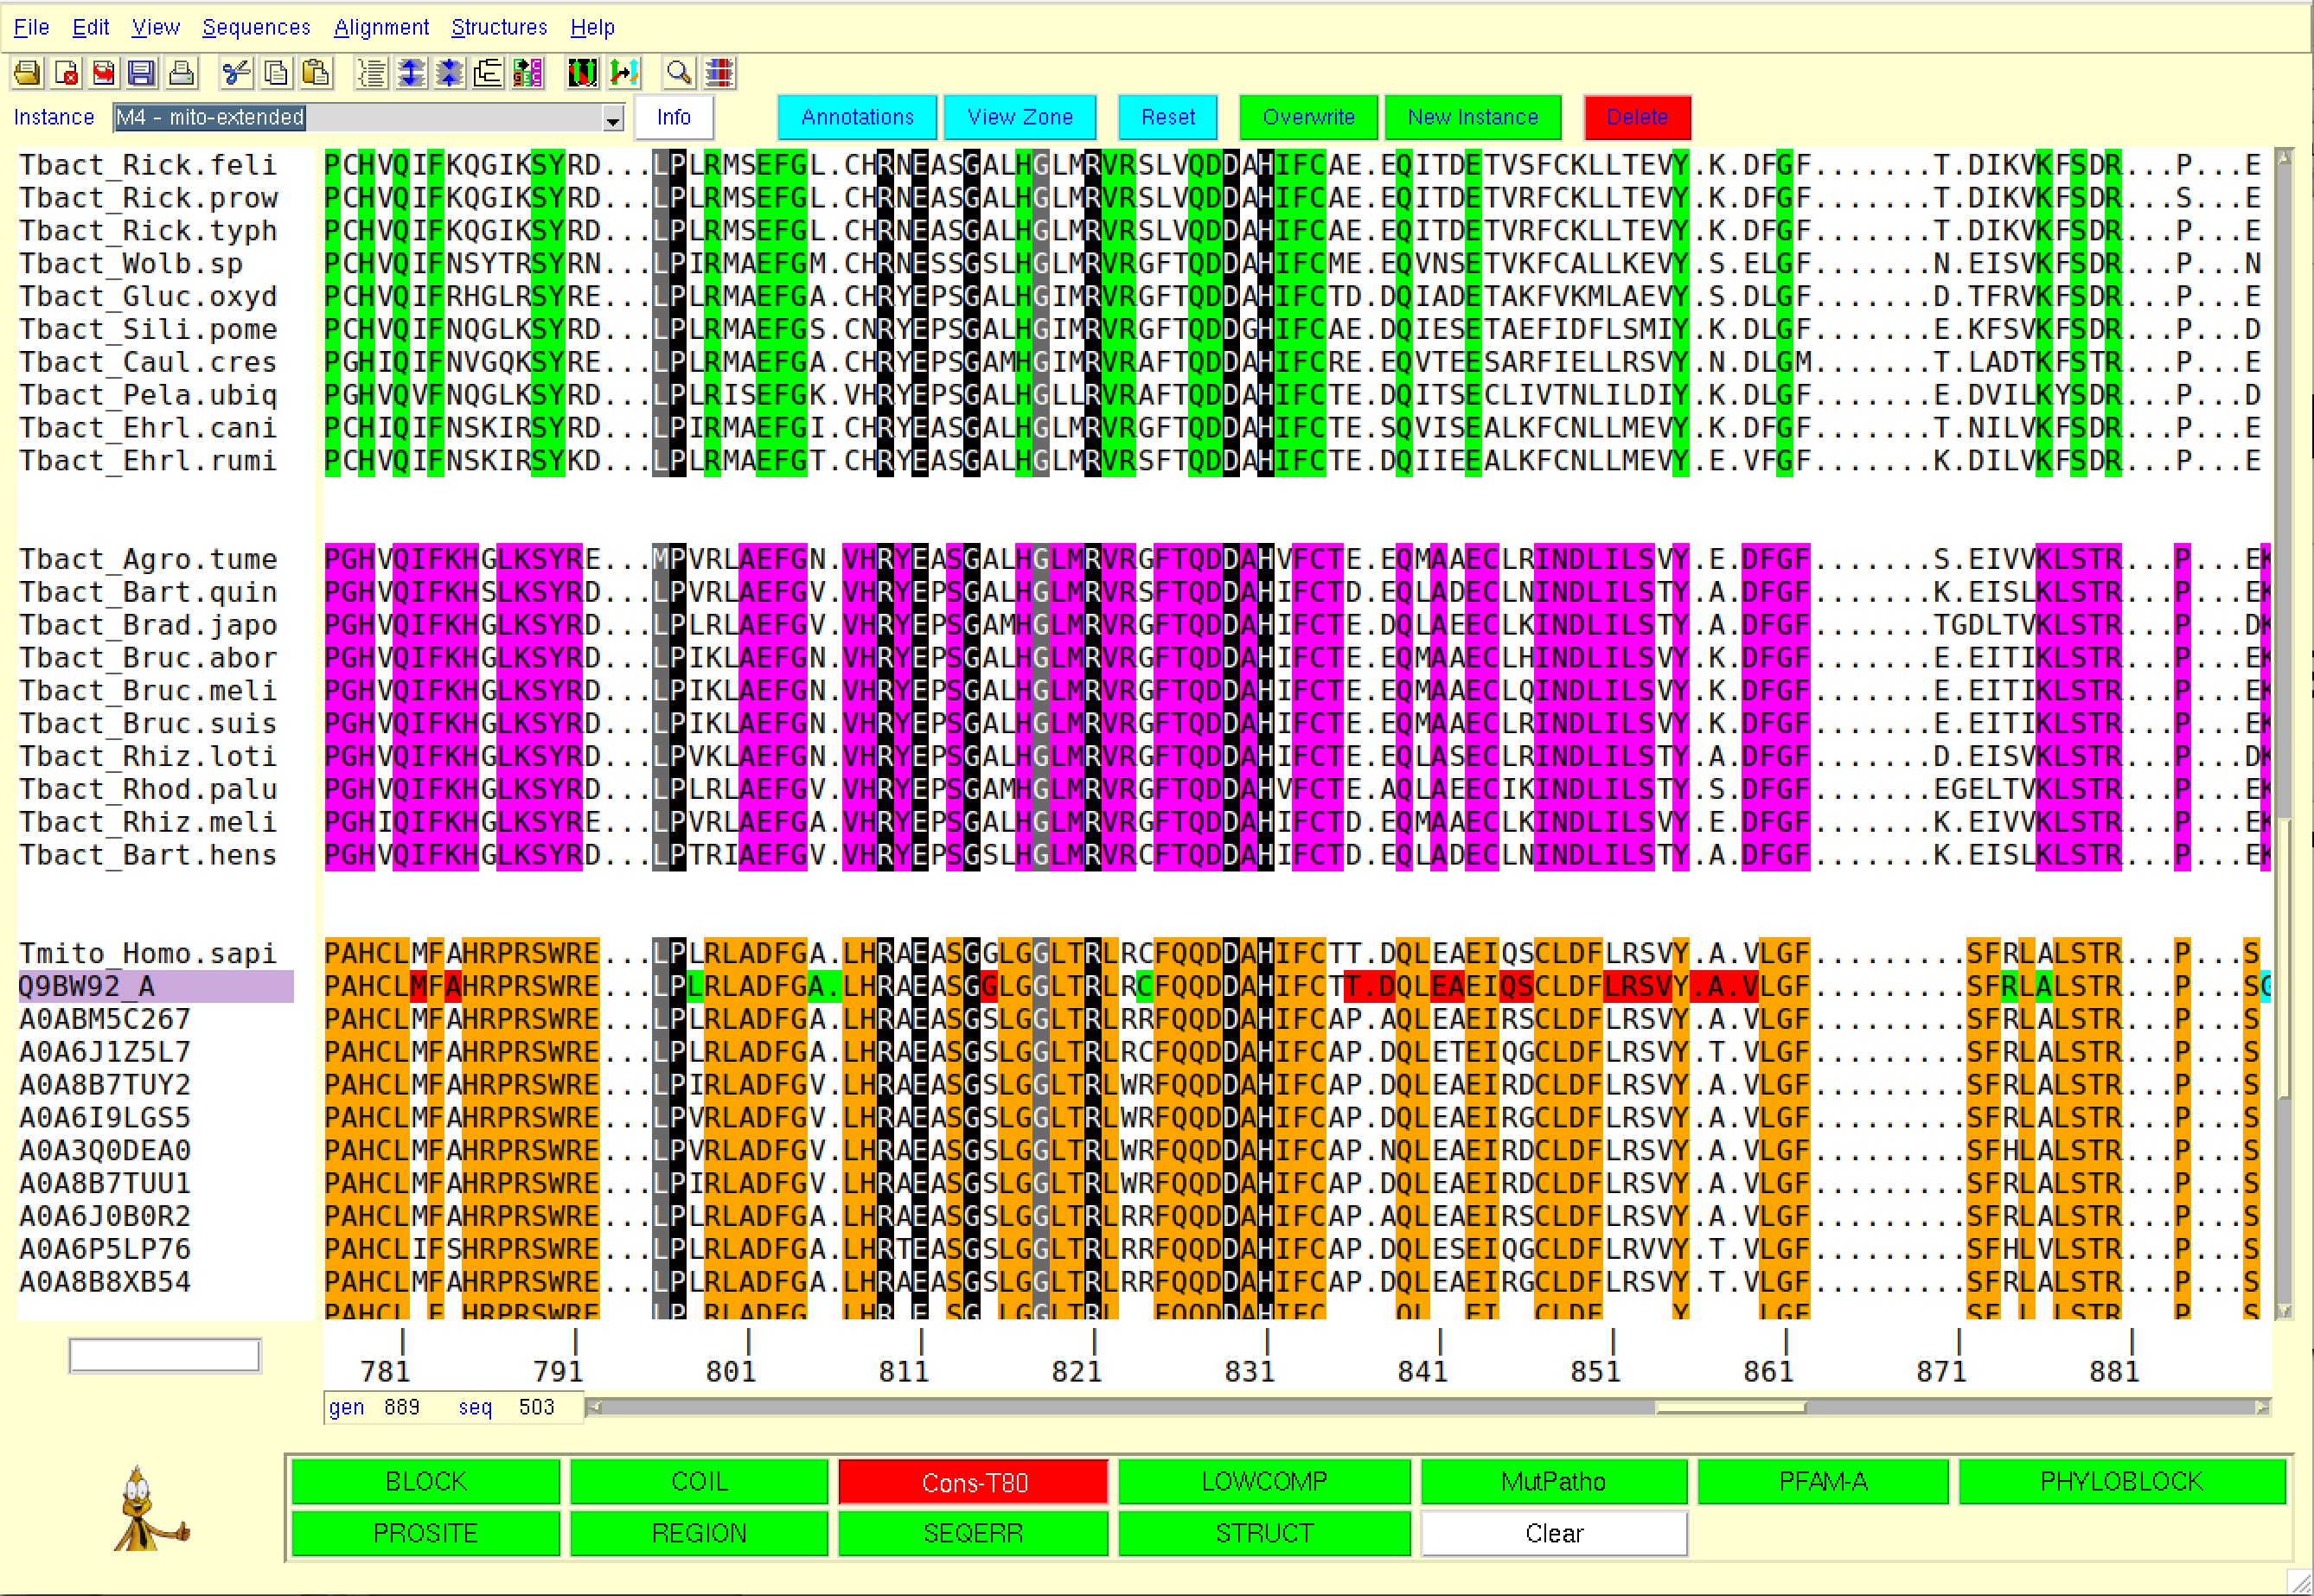
\includegraphics[width=\textwidth, keepaspectratio=true]{ordalie_mainwindow.jpeg}
\caption{Ordalie main window}
\label{mainwindow}
\end{figure}

\subsubsection{The Menus and the icons bar}
All the different menus are described in detail in section \ref{chap-menus} of this manual. In short, the ``File'' menu manages input/output files, as well as printing. The ``Edit'' gives access to the common cut/copy/paste options and to the Preferences. The ``View'' menu controls the appearance of the user interface. It contains options to toggle on or off parts of the main window, to change the font size, or to toggle the full-screen mode. The ``Sequences'' menu allows changing the sequence names, browse, edit or retrieve sequence information, search for sequence motif, compute sequences identity, add sequences or structures coming either from databases or from a file to the current instance. The ``Alignment'' menu gives access to all tools linked to the alignment: alignment editor, clustering, phylogenetic tree, features editor, ... The ``Structures'' menu is dedicated to the structural analysis of the alignment if any sequence corresponding to a 3D structure is present. The menu gives access to a structure superposition module, the 3D viewer, a secondary structure colouring scheme according to sequence conservation, and allows saving PDB files. Finally, the ``Help'' menu allows the access to the on-line documentation and Ordalie version information.
\smallskip
Below the menus, the icon bar gives direct access to some of the most useful menu items, with a tooltip appearing on mouse hover.

\subsubsection{Keyboard shortcuts}
\label{shortcuts}
From the main window (outside any tool), the tools can be launched with the following keys (upper-case letters, i.e.\ \texttt{<Shift>} + letter):
\begin{table}[h!]
\centering
\begin{tabular}{|l|l||l|l|}
\hline
\textbf{Key} & \textbf{Tool} & \textbf{Key} & \textbf{Tool}\\
\hline
\texttt{A} & Annotation        & \texttt{M} & Search Motif\\
\texttt{C} & Conservation      & \texttt{O} & Overview\\
\texttt{E} & Editor            & \texttt{Q} & Toggle physicochemical colouring\\
\texttt{F} & Features display  & \texttt{S} & Superposition\\
\texttt{G} & Clustering        & \texttt{T} & Tree building\\
\texttt{I} & Identity          &            & \\
\hline
\end{tabular}
\caption{Tool shortcuts.}
\end{table}

Other shortcuts:
\begin{itemize}
  \item \texttt{<Ctrl> + <s>}: save the alignment (same as \texttt{File} $\rightarrow$ \texttt{Save});
  \item \texttt{<Ctrl> + <+>} / \texttt{<Ctrl> + <->}: bigger / smaller font;
  \item \texttt{<Ctrl> + <F1>}: toggle full-screen mode;
  \item \texttt{<F2>}: hide/show everything but the alignment (menus, icon bar, instance bar, scores and control panel);
  \item \texttt{<Alt> + <F4>}: quit Ordalie;
  \item \texttt{<Left>}, \texttt{<Right>}, \texttt{<Up>}, \texttt{<Down>}, possibly preceded by a number: scroll the alignment (see the \textit{Navigation tip} in section~\ref{instance-frame}).
\end{itemize}

\subsubsection{The Instance Bar}
\label{instance-bar}
Located above the alignment, this bar allows you to:
\begin{itemize}
  \item Switch between instances (i.e.\ the different analytical scenarios) via a dropdown menu. If the current instance has unsaved changes, Ordalie asks whether to overwrite it, to save the changes as a new instance, to leave it without saving (\textit{Leave without saving}: the changes are discarded, and the instance is unchanged when you come back to it), or to cancel.
  \item View the information attached to the current instance (\textit{Info}): title, description, number of sequences, length, and the name, method and residue zone of its clustering.
  \item Show or hide the annotations of the instance (\textit{Annotations}, see section~\ref{tool-annotate}).
  \item View the zones that lead to the current clustering (\textit{View Zone}).
  \item Reload the current instance, discarding unsaved changes (\textit{Reset}).
  \item Save changes to the current instance (\textit{Overwrite}) or create a new one (\textit{New Instance}). A title and a description are asked for a new instance.
  \item Delete the current instance (\textit{Delete}), after confirmation. Everything that depends on it is deleted too: its data in the database (sequences order, features, clustering, conservation scores, annotations), and the trees and overviews computed on it. The previous instance of the list is then displayed. The instances are not renumbered: deleting M3 of M1 to M4 leaves M1, M2 and M4, and the next new instance is M5. The original alignment (M1) can not be deleted.
\end{itemize}
Switching, resetting, overwriting, creating or deleting an instance is only possible in the main view ('Normal' mode): leave the current mode first (with its \textit{Return}, \textit{Dismiss} or \textit{Cancel} button, depending on the mode). What a mode keeps when it is left becomes a change of the instance, saved with \textit{Overwrite} or \textit{New Instance}, or when switching instance or saving the file.

\subsubsection{The Instance Frame}
\label{instance-frame}
This is the primary workspace, divided into the \textbf{Sequence Names} (left) and the \textbf{Alignment View} (right).

\idee{\texttt{<Mouse-wheel>} scrolls the view vertically, and \texttt{<Ctrl> + <Mouse-wheel>} horizontally, over the sequence names as well as over the alignment. The number of lines and columns scrolled by each wheel step is set in \texttt{Edit} $\rightarrow$ \texttt{Preferences} (\textbf{General} page).}

\paraluc{Sequence Names Pane}
Sequence names associated with a PDB structure are highlighted with a light purple background. Pressing the right mouse button (\texttt{<B3>}) on a name displays, as long as the button is held, the accession number, database ID, organism, sequence length and full description of the sequence, whether imported from Macsim/XML and ORD files or retrieved online (see \ref{tool-inforetrieve}).
\smallskip
Directly below the names list, a search box allows you to find sequences by name or name fragment (case-insensitive; regular expressions are allowed). Pressing \texttt{<Return>} scrolls the alignment to put the first match at the top of the window; pressing \texttt{<Return>} again jumps to the next match.

\paraluc{Alignment View Panel}
The right side of the frame displays the amino acid sequences, accompanied by a ruler at the bottom to indicate column positions. Navigation is managed through horizontal and vertical scrollbars. As you move the mouse over the alignment, the \textbf{position counter} updates in real-time to show two distinct coordinates for the residue currently under the pointer:

\begin{itemize}
    \item \textbf{The 'seq' (Local) position:} This indicates the specific position of the residue within its own individual sequence (excluding gaps).
    \item \textbf{The 'gen' (Global) position:} This represents the absolute coordinate of the residue within the current instance grid.
\end{itemize}

\idee{In this manual, the position within the sequence is referred to as the \emph{local position}, while the position within the instance is referred to as the \emph{global position}.}

When features are displayed, moving the mouse over a feature shows its note. Where several features overlap, a double click (\texttt{<B1>}) brings the feature under the pointer to the front.

\smallskip
\textbf{Navigation tip:} the arrow keys scroll the alignment by one column or one line. Typing a number before an arrow key, on the keyboard or on the keypad, scrolls by that number of columns or lines: for example, \texttt{200} followed by \texttt{<Right>} scrolls 200 columns to the right, \texttt{10} followed by \texttt{<Down>} scrolls 10 lines down. A mouse click or \texttt{<Escape>} cancels a number typed by mistake. This also works while a tool is active (Identity, Clustering, Tree, ...); in the Editor, the cursor itself is moved (see section~\ref{tool-editor}). The mouse pointer must be over the alignment or over the sequence names.

\subsubsection{The Scores Frame}
The Scores frame is hidden by default but can be toggled via the \texttt{View -> Show/Hide scores} menu. Once residue conservation has been computed, a score is assigned to every column of the instance. 

These scores are normalized between 0 and 100 and displayed graphically:
\begin{itemize}
    \item \textbf{Global level:} Represented by a \textbf{black line}, reflecting the conservation across the entire instance.
    \item \textbf{Group level:} If sequence groups are defined, their specific conservation scores are displayed using lines that match their respective \textbf{group colors}.
\end{itemize}

This overlay allows for an immediate visual comparison between family-wide hallmarks and group-specific constraints.

\subsubsection{The Control Panel}
The Control Panel is located at the bottom of the main window. In its default state, the frame displays a welcome message. However, as the analysis progresses, this area becomes a dynamic interface populated with buttons representing the available \textbf{features} of the current instance.

\paragraph{Feature Visibility:}
Each button acts as a toggle for a specific feature:
\begin{itemize}
    \item \textbf{Activation (Red):} Pressing a button turns it \textbf{red} and displays the corresponding feature on the alignment.
    \item \textbf{Deactivation (Green):} Pressing the button again turns it \textbf{green} and removes the feature from the view.
    \item \textbf{Clear:} hides all the displayed features at once.
\end{itemize}
Buttons of conservation score features are initially yellow instead of green.

\idee{The features are rendered in the order their buttons are activated. To change the layering (e.g., to place a specific domain on top of a conservation score), simply toggle the buttons to reorder the display stack!}

\paragraph{Contextual Adaptation:}
The content of the Control Panel is context-sensitive. When switching between different Ordalie tools (e.g., from the Editor to the Clustering tool), the panel will automatically update to show the controls specific to that module. Detailed descriptions of these specific controls are provided in their respective sections of this manual.

\subsection{Features}
\textbf{Features} are a central pillar of the Ordalie architecture. A feature is defined as a biological or structural characteristic mapped onto a specific coordinate range. These can be categorized by their scope:

\begin{itemize}
    \item \textbf{Sequence Features:} Specific to a single sequence (e.g., a PTM site or a single PFAM domain).
    \item \textbf{Group Features:} Characteristics shared by a specific cluster of sequences.
    \item \textbf{Global Features:} Hallmarks applicable to the entire instance or protein family.
\end{itemize}

A single feature can encompass multiple \textit{items}; for example, a "Domains" feature may contain several distinct PFAM occurrences along the sequence. One of the primary strengths of Ordalie is its ability to investigate these features across multiple dimensions, such as projecting sequence-based motifs directly onto 3D structures.

\subsubsection{Data Provenance}
Features can be integrated into Ordalie through three main channels:
\begin{enumerate}
    \item \textbf{External software:} Parsing XML output from the Macsims program \cite{soft:macsims}.
    \item \textbf{Dedicated files:} Using the Ordalie feature file format (see section \ref{chap-featurefile}).
    \item \textbf{Manual curation:} User-defined annotations created via the \textit{Features Editor} tool (see \ref{tool-feateditor}).
\end{enumerate}

\attention{Ordalie does not automatically generate biological features. The only exception is the \textbf{Conservation Tool}, which creates new feature items based on each calculated conservation score.}

\newpage
\section{Ordalie Tools}
\label{chap-tools}

Ordalie contains a collection of tools that can be called at any time. Tools that change the display of the alignment (Editor, Identity, Clustering, Tree, Conservation, Superposition, Features Editor, Annotation) are exclusive: leave the current one (\textit{Return}, \textit{Save} or \textit{Cancel}) before starting another one. Window tools (Overview, Features Summary, Barcode, 3D Viewer, trees) can stay open at any time.

\subsection{Instance Overview}
\label{tool-overview}
The \textit{Instance Overview} provides a condensed, schematic representation of the entire alignment. This tool is designed to facilitate navigation and global feature inspection. Multiple overview windows can be opened simultaneously for the same instance, allowing for different levels of zoom or feature mapping.

\begin{figure}[h!]
\centering
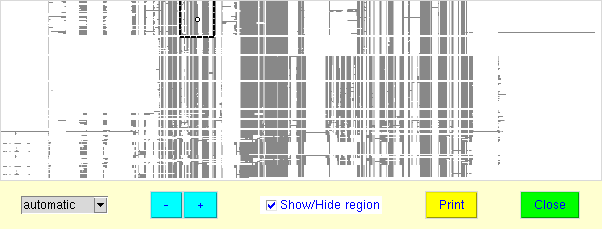
\includegraphics[width=\textwidth, keepaspectratio=true]{overview.png}
\caption{The Instance Overview tool window, showing the alignment scheme and control panel.}
\label{fig-overview}
\end{figure}

\subsubsection{The Instance Frame}
In this view, the alignment is abstracted: each residue is represented by a single grey pixel on a white background. This miniaturized "map" provides two main interactive functions:

\begin{itemize}
    \item \textbf{Feature Mapping:} Any sequence or global feature can be overlaid onto this scheme, highlighting motifs or domains across the whole family.
    \item \textbf{Navigation \& Synchronization:} A \textbf{stippled rectangle} (bounding box) indicates the region currently visible in the main alignment window. Clicking anywhere on the scheme will instantly center the main window on that specific position.
\end{itemize}

\subsubsection{Control Panel}
The control panel at the bottom of the window manages the display and interaction (fig. \ref{fig-overview}):

\begin{itemize}
\item \textbf{Feature Selector (Combobox):} By default, this is set to \textbf{'automatic'}, meaning the Overview reflects exactly what is displayed in the main window. Selecting a specific feature here will force its display on the Overview independently of the main window settings. Selecting \textbf{None} removes any feature from the Overview.
    \item Zoom (\textbf{+} / \textbf{-}): These buttons adjust the scale of the schematic pixels, allowing the user to switch between a dense family-wide view and a more detailed motif-level view.
    \item \textbf{Show/Hide region:} shows or hides the rectangle marking the part of the alignment visible in the main window.
    \item \textbf{Annotations:} shows or hides the annotations of the instance (see section \ref{tool-annotate}) as rectangles of their color, drawn above the features. Hovering over a rectangle shows the text of the annotation. The box is checked when the Overview is opened if the \textit{Annotations} button of the instance bar is pressed. The Overview is updated when the Annotation tool is left with \textit{Return}.
    \item \textbf{Print:} Exports the current schematic state as a PNG image. The software will prompt for a destination file name.
    \item \textbf{Close:} Closes the Overview window.
\end{itemize}

The overviews open when an ORD file is saved are saved with it, whatever their instance, and are drawn again when the file is opened, with the same settings (feature selector, features shown, zoom, region and annotations boxes). The trees of all the instances are drawn again as well. Each one is computed on the alignment of its instance: to do so, Ordalie displays the instances that have trees or overviews in turn while the file is opened, then comes back to the current instance. The trees and overviews of an instance are deleted with it (\textit{Delete} button of the instance bar, section \ref{instance-bar}).

\subsection{Editor}
\label{tool-editor}
The quality of downstream analyses (phylogeny, conservation, or feature mapping) is strictly dependent on the accuracy of the Multiple Sequence Alignment (MSA). While automated algorithms are highly advanced, manual curation remains an essential step. Ordalie integrates a high-performance sequence editor inspired by the \textit{SeqLab} interface (GCG Wisconsin Package), designed for intuitive and precise alignment refinement.

\smallskip
Upon entering the Editor, sequences are automatically colored according to their physico-chemical properties. 

\begin{figure}[h!]
\centering

\includegraphics[width=\textwidth, keepaspectratio=true]{aa_colouring_scheme.png}
\caption{Default physico-chemical amino acid coloring scheme in the Editor.}
\end{figure}

\textit{Note: The default coloring scheme can be customized in the \texttt{Edit -> Preferences} menu. Active features remain visible on the instance to guide the editing process.}

\attention{To ensure data consistency, some analytical functionalities are temporarily disabled while the Editor tool is active.}

\subsubsection{Control Panel}
The Editor control panel at the bottom of the window provides the following management tools:

\begin{description}
\item \textbf{Clear selections:} Deselects all currently selected sequences.
    \item \textbf{Group / Ungroup:} Groups the selected sequences. Grouped sequences are assigned a unique name color; the group-wide editing commands (\texttt{<Shift-Space>}, \texttt{<Shift-Backspace>}, see below) then act on all members of the group.
    \item \textbf{Lock / Unlock:} By default, the editor is \textbf{Locked}, meaning only gap characters (\texttt{.}) can be inserted or deleted. Unlocking the sequences allows for the direct insertion or deletion of amino acid residues. The initial state is set in \texttt{Edit} $\rightarrow$ \texttt{Preferences} (\textbf{Editor} tab).
    \item \textbf{Map/Unmap residues:} A toggle to enable or disable the physico-chemical color scheme.
    \item \textbf{Remove columns of gaps:} Scans the instance and deletes any columns consisting entirely of gaps. This operation is also performed automatically upon exiting the Editor.
    \item \textbf{Show feature / Hide features:} the menu button lists all features as check buttons, to toggle specific features on or off (features are layered in the order they are activated); \textit{Hide features} removes all of them from the display.
    \item \textbf{Temp. save} (\texttt{<Ctrl> + <t>}): writes the current state of the alignment to a FASTA (\texttt{.tfa}) file. This acts as a manual checkpoint during long editing sessions. The file name is asked the first time only; subsequent temporary saves overwrite the same file.
    \item \textbf{Search Motif:} Switch to the search motif tool, see \ref{tool-motif}.
    \item \textbf{Save \& Return:} Exits the editor and prompts the user to either overwrite the current instance or create a new one with the changes.
    \item \textbf{Cancel:} Exits the editor and discards all changes, restoring the instance to its original state.
\end{description}

\subsubsection{Edition Actions}
Clicking within the alignment frame activates a \textbf{yellow blinking cursor}. The following keyboard interactions are then available:

\begin{itemize}
    \item \textbf{Navigation:} Use the \texttt{Arrow} keys to move the cursor through the alignment grid.
    \item \textbf{Gap insertion:} \texttt{<Space>} inserts a gap (\texttt{.}) at the cursor in the current sequence; \texttt{<Shift-Space>} inserts it in all sequences of the group of the current sequence.
    \item \textbf{Deletion:} \texttt{<Backspace>} removes the character preceding the cursor; \texttt{<Shift-Backspace>} does the same for all sequences of the group. \textit{Reminder: In Lock mode, only gaps can be deleted.}
    \item \textbf{Residue insertion:} when the sequences are unlocked, typing an amino acid letter inserts it at the cursor.
    \item \textbf{Shifting (The "Push" mechanism):} 
    \begin{itemize}
        \item \texttt{<Shift-Right>}: Pushes the block of contiguous residues to the right of the cursor until the next common gap.
        \item \texttt{<Shift-Left>}: Pushes the block of contiguous residues to the left of the cursor until the previous common gap.
    \end{itemize}
\end{itemize}



\paragraph{Numeric Buffer (Rapid Navigation):} 
To speed up editing, you can type a number (0-9) before a command. The digits are stored in a buffer (e.g., typing \texttt{1} then \texttt{2} stores \texttt{12}). Pressing a navigation or shift key will then apply that action \texttt{12} times and clear the buffer. The buffer applies to arrows, push, gap insertion, deletion and residue insertion. Digits can be typed on the main keyboard or on the keypad (with or without NumLock). The cursor stops at the first/last column and at the first/last sequence, and the sequence names and the ruler follow the view. A mouse click or \texttt{<Escape>} empties the buffer.

\subsection{The Identity Tool}
\label{tool-identity}
The Identity tool provides quantitative data on the sequence identity percentages within the instance. It allows for precise comparisons between specific sequences or defined residue ranges (features), making it essential for characterizing sub-family divergence or domain-specific conservation.

\begin{figure}[htbp]
\centering
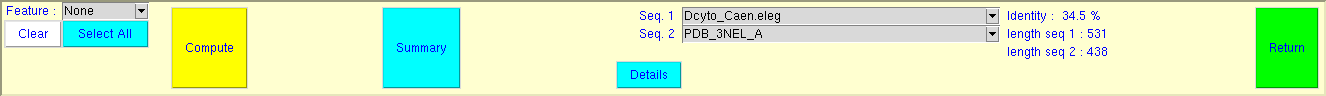
\includegraphics[width=\textwidth, keepaspectratio=true]{identity_controlpanel.png}
\caption{The control panel of the Identity tool.}
\end{figure}

\subsubsection{Control Panel}

The interface is divided into selection management on the left and computation/results on the right.

\paragraph{Selection Management}
Before computing identity, the user must define the scope of the analysis:
\begin{itemize}
    \item \textbf{Feature:} a dropdown menu to display a feature (e.g.\ a domain); its items can then be selected as residue ranges with \texttt{<Ctrl> + <B1>}, or with \texttt{<B1>}/\texttt{<B3>}.
    \item \textbf{Clear:} Resets all current sequence and residue range selections.
    \item \textbf{Select All:} Automatically selects the entire length of all sequences in the instance.
\end{itemize}

\paragraph{Computation and Results}
Once the scope is defined, the following actions are available:

\begin{description}
    \item[Compute:] Triggers the identity calculation. A detailed summary is automatically sent to the \textbf{Log Console}, see \ref{viewlog}. 
    \item[Summary:] Opens a new window providing aggregate statistics for the entire selection and for each individual group:
    \begin{itemize}
        \item The \textbf{average identity percentage}.
        \item The \textbf{standard deviation}.
        \item Identification of the pairs with the \textbf{maximum} and \textbf{minimum} identity percentages.
    \end{itemize}
  \item[Pairwise Comparison:] Using the two dedicated comboboxes, the user can select any two sequences to display their specific identity percentage and the length of the ungapped sequences compared.
  \item[Details:] Opens a new window providing detailed information for the selected sequence pair. The identity percentage and sequence lengths are displayed. For each sequence, its most identical (closest) and most distant sequences are specified, along with their respective identity percentages. If the instance is clustered, the window also highlights the closest and most distant sequences both within and outside the sequence's cluster (see figure~\ref{identity-details}).
    \item[Return:] Exits the Identity tool and returns to the main window.
\end{description}

\begin{figure}[htbp]
\centering
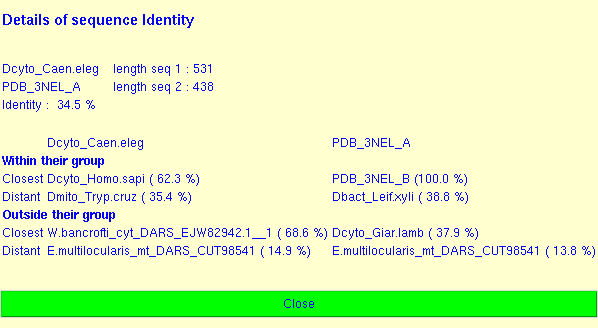
\includegraphics[width=0.5\textwidth, keepaspectratio=true]{identity_details.png}
\caption{The ``Details'' window}
\label{identity-details}
\end{figure}

\subsection{The Search Motif Tool}
\label{tool-motif}
The Search Motif tool allows for rapid identification of specific sequence patterns within the current instance.

\begin{figure}[htbp]
\centering
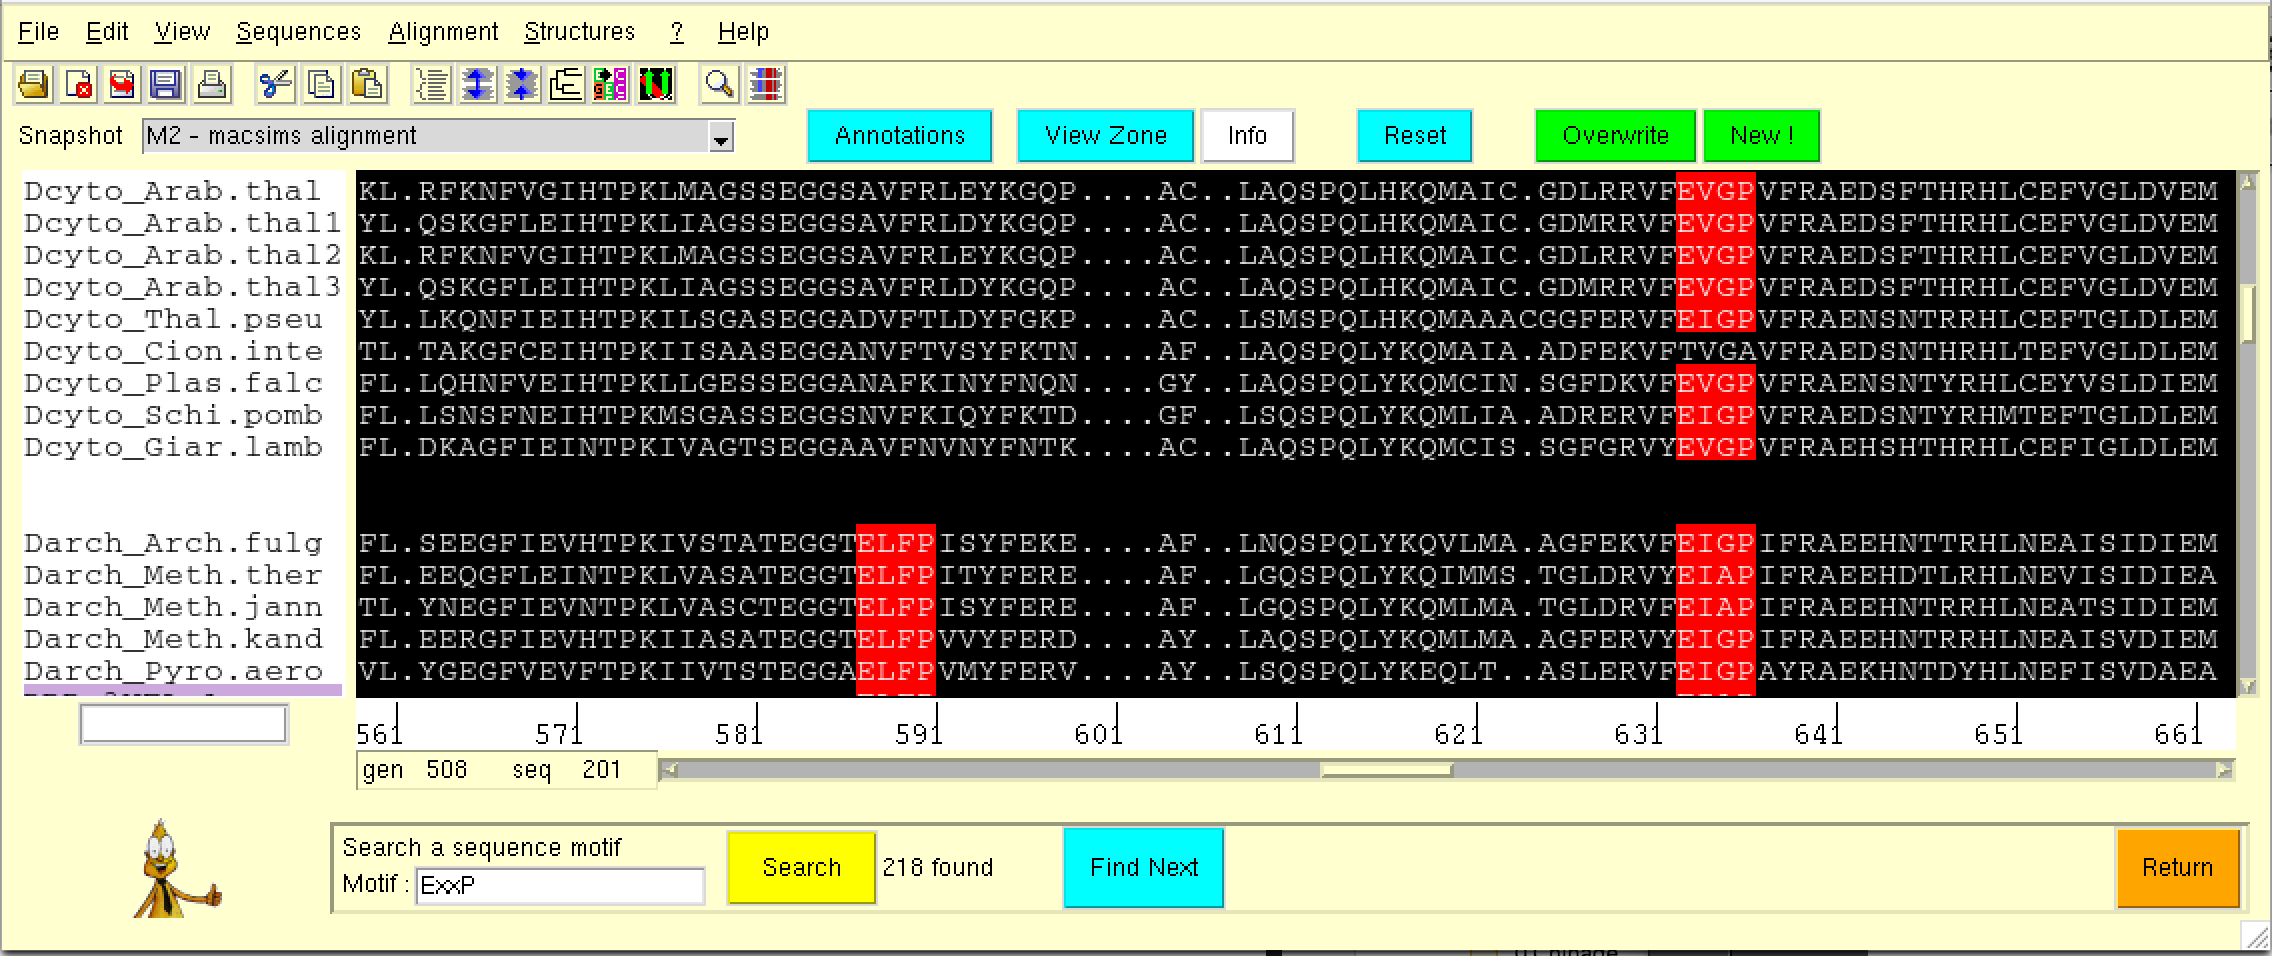
\includegraphics[width=\textwidth, keepaspectratio=true]{search.png}
\caption{The Search Motif tool in action. Detected occurrences are highlighted in red against a high-contrast black background.}
\end{figure}

\subsubsection{Search Pattern Syntax}
Ordalie adopts the robust \texttt{FindPatterns} syntax from the GCG Wisconsin Package \cite{soft:gcg}. This allows for complex queries, including ambiguous residues and variable-length gaps. A comprehensive guide to this syntax is provided in Appendix \ref{findpatterns}.

\subsubsection{Control Panel}
The Search Motif interface is minimalist and designed for speed:

\begin{description}
    \item[Motif Entry Box:] The text field where the search pattern is defined.
    \item[Search:] Launches the initial scan across all sequences in the instance.
    \item[Find Next:] Navigates the view to the next occurrence of the motif.
    \item[Return:] Exits the search tool and restores the standard display.
\end{description}

The motif is searched in the sequences without their gaps, so an occurrence can span gaps of the alignment. The search is case-insensitive. The number of occurrences found is displayed next to the \textbf{Search} button. Pressing \texttt{<Return>} in the motif entry box also launches the search.

\paragraph{Visual Feedback:} 
When a search is successful, Ordalie switches to a high-contrast mode: the instance background turns \textbf{black}, and every occurrence of the found motif is highlighted in \textbf{red}. This visual "negative" ensures that even single-residue motifs are easily spotted in large alignments.

\attention{The ``Search Motif'' is the only tool that remains accessible while the \textbf{Editor} tool is active, facilitating real-time curation based on specific motif locations.}

\subsection{The Clustering Tool}
\label{tool-clustering}

The \textbf{Clustering} tool enables the grouping of sequences based on numerical criteria derived from sequence characteristics. The computation can integrate all or part of the sequence, as well as specific instance columns. Users can combine multiple numerical criteria and select a specific clustering algorithm. 

Once launched, the newly created sequence clusters are automatically displayed in the main window. While clustering trials are stored temporarily during the session, any specific clustering result can be permanently saved as a new instance.

\subsubsection{Criteria}
The tool currently supports the following numerical criteria:

\begin{itemize}
    \item \textbf{Identity percentage}: Calculated for each sequence over the selected residue range against all other selected sequences.
    \item \textbf{Length}: The total length of the sequence.
    \item \textbf{Hydrophobicity}: mean hydrophobicity of the sequence, computed with the GES (Engelman) scale.
    \item \textbf{Isoelectric point (pI)}: Computed using the EMBOSS pKa values for amino acids.
    \item \textbf{Amino acid composition}: The relative percentage of the 20 standard amino acids within a given sequence.
\end{itemize}

\subsubsection{Algorithms}
Ordalie automatically determines the optimal number of groups. The clustering algorithms and the methods for defining cluster counts are integrated from the \textbf{Cluspack} package. Available methods include:

\begin{itemize}
    \item \textbf{K-means / DPC (Density of Points Clustering)} \cite{dpc}: Cluster identification is based on point density criteria, while the final selection is performed via the k-means algorithm.
    \item \textbf{Hierarchic / Secator} \cite{secator}: Groups are identified through ascending hierarchical classification. Cluster selection is determined by an inertia loss criterion.
    \item \textbf{Mixture Model} \cite{mixturemodel} / \textbf{AIC} \cite{aic} or \textbf{BIC} \cite{bic}: Data distribution is modeled using Gaussian distributions, with clustering optimized according to the Akaike Information Criterion (AIC) or the Bayesian Information Criterion (BIC).
\end{itemize}

\subsubsection{Control Panel}
\begin{figure}[h!]
    \centering
    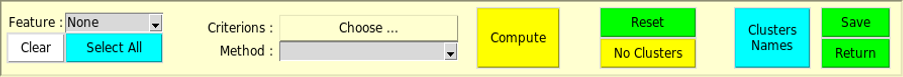
\includegraphics[width=\textwidth, keepaspectratio=true]{clusters_controlpanel.png}
    \caption{The Clustering tool control panel interface.}
\end{figure}

\paragraph{Selections}
The left section of the Control Panel manages sequence and residue range selection:
\begin{itemize}
    \item \textbf{Feature}: Displays the chosen feature. Users can select one or more items from this feature (\texttt{<Ctrl> + <B1>}) to define a residue range.
    \item \textbf{Clear}: Resets all previously selected residue ranges and sequences.
    \item \textbf{Select All}: Selects all columns in the current instance.
\end{itemize}

\textit{Note on selections:} if no residue range is selected, the whole alignment is used. If no sequences are selected, the tool processes \textbf{all} sequences. If more than 3 sequences are selected, the clustering applies only to them and unselected sequences are grouped into a separate "Others" category. At least 3 sequences must have residues in the selected columns.

\paragraph{Clustering criteria}
The pull-down menu allows for the selection of one or more criteria. 

\attention{The special \textbf{'Life domain'} criterion (Eukaryota, Archaea, Bacteria, Viruses) is categorical and cannot be combined with other numerical criteria. It does not require a clustering method.}

\paragraph{Clustering methods}
The 'Method' menu provides access to the algorithms:
\begin{itemize}
    \item Hierarchic clustering / Secator
    \item K-means / DPC
    \item Mixture model / AIC criterion
    \item Mixture model / BIC criterion
\end{itemize}

Clicking \textbf{``Compute''} updates the main Ordalie window with the resulting groups.

\paragraph{Other buttons}
\begin{itemize}
    \item \textbf{Reset}: Reverts to the clustering stored in the file (only available for Macsim/XML and ORD alignments).
    \item \textbf{No Clusters}: Removes all existing groups, merging all sequences into a single block.
    \item \textbf{Clusters Names}: Opens a dialog to rename clusters. These names are preserved in other modules, such as the \textbf{Barcode} tool.
    \item \textbf{Save}: Ends the session and saves the results in the instance. You will be prompted to either overwrite the current instance or create a new one.
    \item \textbf{Return}: Exits the tool without saving changes, restoring the instance to its initial state.
\end{itemize}

\subsection{The Tree Tool}
\label{tool-tree}

The \textbf{Tree} tool is divided into two main phases: tree construction, performed within the main Ordalie window, and tree exploration, which takes place in a dedicated visualization window.

The tree is computed using the \textbf{FastME} program \cite{soft:fastme} with default parameters. Ordalie first generates a distance matrix based on identity percentages calculated over the selected residue range (the distance between two sequences is $1 - \mathrm{identity}$). A residue range must be selected before drawing the tree, and at least 10 alignment columns must remain after gap removal. While Bayesian-based algorithms can offer higher precision, FastME provides an excellent balance between computational speed and phylogenetic accuracy.

\subsubsection{Control Panel for Tree Building}
\label{control-tree}

\begin{figure}[htbp]
    \centering
    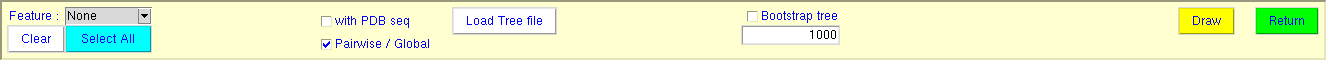
\includegraphics[width=\textwidth, keepaspectratio=true]{tree_controlpanel.png}
    \caption{The Tree building tool control panel.}
\end{figure}

\paraluc{Selections}
The left section of the Control Panel manages sequence and residue range selection:
\begin{itemize}
    \item \textbf{Feature}: Displays the chosen feature. Users can select one or more items from this feature (\texttt{<Ctrl> + <B1>}) to define the residue range for computation.
    \item \textbf{Clear}: Resets all previously selected residue ranges and sequences.
    \item \textbf{Select All}: Selects all residue columns from the entire alignment.
\end{itemize}

\paraluc{Options}
The following settings control the tree computation process:
\begin{itemize}
    \item \textbf{With PDB seq}: Includes PDB sequences in the computation. By default, Ordalie excludes them as they are typically redundant with existing sequences in the instance.
    \item \textbf{Pairwise / Global}: Defines the gap removal strategy. \textit{Pairwise} (checked) excludes gaps on a per-pair basis during distance calculation. \textit{Global} (unchecked) uses only complete columns (without any gaps) for the entire computation.
    \item \textbf{Load Tree file}: imports and displays an external tree file in \textbf{Newick} format. Leaf identifiers must match the sequence names present in the instance. Imported trees have no bootstrap values.
    \item \textbf{Bootstrap tree}: when checked, Ordalie performs \textit{N} bootstrap replicates, \textit{N} being typed in the entry box next to the check button (default 1000, standard value for publication).
\end{itemize}

\paraluc{Draw / Return}
The \textbf{``Draw''} button launches the computation and opens the tree in a new window. The \textbf{``Return''} button exits the Tree tool.

\subsubsection{The Tree Visualization Window}
Each newly computed tree is rendered in a dedicated window designed for deep exploration of phylogenetic characteristics. Ordalie supports two primary visualization modes: \textbf{Dendrograms} (rectangular layouts) and \textbf{Radial Trees} (circular layouts). While most options are universal, some are tailored to a specific representation.

\begin{figure}[h!]
    \centering
    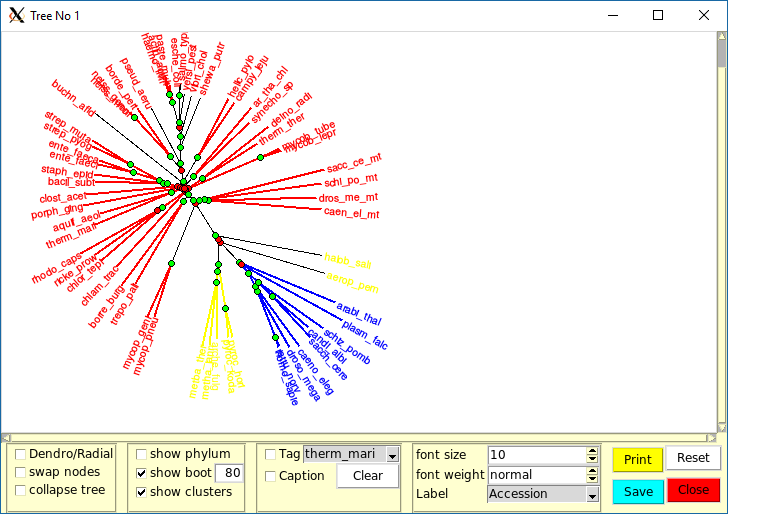
\includegraphics[width=\textwidth, keepaspectratio=true]{TreeWindow.png}
    \caption{The Tree rendering window. In this radial view, nodes are marked with circles indicating if bootstrap values exceed (green) or fall below (red) the user-defined threshold. Sequences are color-coded by cluster.}
\end{figure}

The interface is divided into a large \textbf{Drawing Area} (top) and a comprehensive \textbf{Control Panel} (bottom).

\paraluc{The Drawing Area}
This interactive area allows for direct manipulation of the tree:
\begin{itemize}
    \item \textbf{Navigation}: Move the entire tree by dragging it with the mouse (Button-1).
    \item \textbf{Scaling \& Scrolling}: In a \textit{Radial Tree}, the mouse wheel scales the diagram. In a \textit{Dendrogram}, the wheel scrolls vertically through the sequences.
    \item \textbf{Customization}: A right-click (Button-3) opens a contextual menu: for dendrograms it changes the width and the height of the tree; for radial trees it zooms and rotates the tree. The \textit{Pointer} entry returns to the normal mouse behaviour.
\end{itemize}

\paraluc{The Control Panel}
The panel is organized into four functional groups to streamline the analysis:

\noindent\textbf{1. General Tree Options}
\begin{itemize}
    \item \textbf{Dendrogram/Radial}: Switches the graphical representation of the tree.
    \item \textbf{Swap Node}: Enables orange markers at each node; clicking a marker rotates the descendant branches around that node.
    \item \textbf{Re-root Tree} (Dendrogram only): Enables green markers at nodes. Clicking a marker sets a new root, effectively redefining the outgroup branches.
    \item \textbf{Collapse Tree} (Radial only, bootstrapped trees only): collapses the branches whose bootstrap value is below the threshold, giving multifurcating nodes. Unchecking it restores the full tree. In a radial tree, this check button replaces \textbf{Re-root Tree}.
\end{itemize}

\textbf{\noindent2. Visual Annotations}
\begin{itemize}
    \item \textbf{Show Phylum}: colours the sequence names according to their life domain (by default pink for Eukaryota, light blue for Archaea, light yellow for Bacteria, black for Viruses; colours set in \texttt{Edit} $\rightarrow$ \texttt{Preferences}, \textbf{Sequences} page). The option is available when the life domain of at least one sequence of the tree is known: it is read from Macsim/XML and ORD files, and can be obtained for any alignment with \texttt{Sequences} $\rightarrow$ \texttt{Retrieve Sequences information} (sequences named with a UniProt or RefSeq accession). Sequences whose life domain is unknown keep a white background.
    \item \textbf{Show Bootstrap}: Displays colored discs at nodes based on a confidence threshold (default 80\%). Green circles represent high confidence, while red indicates lower support. In dendrograms, absolute bootstrap values are printed; in radial trees, they appear as tooltips when hovering over a node. The threshold can be changed in the entry box next to the check button (validate with \texttt{<Return>}). This option is only available when the tree has been bootstrapped.
    \item \textbf{Show Clusters}: If a clustering analysis was previously performed, branches are color-coded to match their respective clusters.
\end{itemize}

\attention{The colors assigned to life domains can be changed using ``Edit -> Preferences'' menu item.}

\noindent\textbf{3. Labels and Metadata}
\begin{itemize}
    \item \textbf{Tag}: Highlights a specific leaf (chosen via the combobox) with a thick black frame for rapid identification.
    \item \textbf{Caption}: opens a window where a free text can be entered and where the elements to be displayed are chosen: gap handling, number of sites, number of bootstrap replicates and threshold, group colours. \textbf{Clear} removes the caption.
    \item \textbf{Font}: Adjusts the font size and weight (Normal/Bold).
    \item \textbf{Labels}: The \textbf{Label} menu selects which metadata to display: Sequence Name, Accession, Bank ID, Organism, Description, or a combination of two of them.
\end{itemize}

\noindent\textbf{4. Global Actions}
\begin{itemize}
    \item \textbf{Print}: Captures the current tree view and exports it as a high-quality PNG file.
    \item \textbf{Save}: saves the tree in Newick format.
    \item \textbf{Reset}: Restores the tree to its default parameters and orientation.
    \item \textbf{Close}: Exits the visualization window.
\end{itemize}


\subsection{The Conservation Tool}
\label{tool-conservation}

Evolutionary pressure, which maintains the structure and function of protein families, leaves detectable traces in residue conservation patterns. Analyzing both global and group-specific conservation helps in identifying key functional sites, such as ligand-binding pockets, protein-protein interaction patches, or residues linked to functional specialization within sub-groups.

Ordalie provides a comprehensive suite of methods to quantify this conservation. Users can experiment with different algorithms, and results are stored temporarily during the session. Once a computation is saved, it is integrated as a new \textbf{Feature} within the instance, making it available for visualization and analysis across all other Ordalie tools.

\subsubsection{Conservation Methods}
Residue conservation can be measured using various established metrics \cite{valdar, johansson}. Ordalie implements several standard algorithms alongside two proprietary methods.

\paragraph{The 'Threshold' Method}
This is a simple frequency-based counting method. Two pre-set thresholds define the levels of conservation:
\begin{itemize}
    \item \textbf{Identity Conservation Threshold}: Set by default to 100\%. Columns reaching this level are flagged as 'Identity conservation'.
    \item \textbf{Global Conservation Threshold}: Set by default to 80\%. Columns meeting this criteria are considered 'Globally conserved'.
\end{itemize}

At the group level, only the Identity threshold is applied. The global conservation threshold can be changed in the \textit{Preferences} (\textbf{Conservation} tab) or with the \texttt{-threshold} command line option; the identity threshold is fixed to 100\%.

\paragraph{Automatic Methods}
These methods follow a two-step statistical approach and only process columns where at least 30\% of the sequences (and at least 3 sequences) have a residue. They require more than 3 sequences; groups containing 3 sequences or less are ignored:
\begin{enumerate}
    \item \textbf{Scoring}: Each column is assigned a raw score based on the chosen algorithm.
    \item \textbf{Clustering}: the column scores are clustered with a Gaussian mixture model (AIC criterion, Cluspack package). Clusters are then ranked by their mean score. The two highest-ranking clusters are designated as 'Strictly conserved' and 'Globally conserved'. For group-specific analyses, only the top-ranking cluster is retained.
\end{enumerate}

Available automatic methods include:
\begin{itemize}
\item \textbf{BILD (Bayesian Inferred Log-Likelihood Divergence)}: A Bayesian scoring method that assesses column conservation by comparing a posterior distribution, derived from Dirichlet mixtures, against a background null model \cite{bild}. It is particularly robust for small alignments as it uses prior biological knowledge to stabilize frequency estimations, making it highly effective for identifying functional motifs with limited data.
\item \textbf{Shannon Entropy}: A classic information-theoretic metric that quantifies the uncertainty or randomness at a specific alignment position \cite{meth:shannona,meth:shannonb}. The score is calculated based on the frequencies of the observed residues in a column; a lower entropy signifies a highly conserved position, while a higher entropy reflects high variability. It serves as the baseline for most evolutionary conservation analyses.
\item \textbf{Liu}: An entropy-based approach proposed by Liu \emph{et al.} \cite{liu2} that quantifies conservation by measuring the reduction in uncertainty at a specific position. Unlike Shannon's classic entropy, this method incorporates sequence weighting or stereochemical properties to better distinguish between purely invariant columns and those exhibiting conservative substitutions.
\item \textbf{Mean Distances}: The matrix-based algorithm popularized by ClustalX \cite{soft:clustalx}. It calculates the average of all pairwise scores between residues in a column using a substitution matrix (e.g., BLOSUM or PAM). This method effectively captures the "average" biochemical similarity.
\item \textbf{JSD (Jensen-Shannon Divergence)}: A powerful information-theoretic metric used to measure the distance between the observed residue distribution in a column and a reference background distribution (e.g., BLOSUM62 frequencies) \cite{method:jsd}. The JSD is symmetric and bounded, providing a normalized score.
\item \textbf{Vector Norm}: A proprietary method that projects amino acids into a multidimensional physicochemical space, primarily defined by properties such as Van der Waals volume and polarity. The score is calculated as the magnitude of the mean property vector in this space; a high norm indicates a strong consensus where residues share similar physical constraints. See Appendix \ref{meth-vectornorm} for the detailed geometric derivation.
\item \textbf{Multi}: A meta-scoring hybrid approach designed to increase the signal-to-noise ratio. By combining orthogonal metrics chosen by the user through a dedicated window, it aggregates complementary methods that do not measure exactly the same properties. The scores of the chosen methods are standardized before being combined.
\end{itemize}

\subsubsection{Specificity-Determining Positions: GroupSim}
\label{tool-groupsim}
Specificity-determining positions are columns that are conserved within each group of sequences but differ between groups, \emph{i.e.} residues potentially responsible for the functional specialization of sub-families. They are predicted by the \textbf{GroupSim} method, below a separator line at the end of the \textbf{Method} menu, with \textbf{Compute}. Ordalie implements the GroupSim+ConsWin method of Capra and Singh \cite{groupsim}, using the groups currently defined as specificity groups (see the Clustering tool, section \ref{tool-clustering}); the computation is fast (less than a second for 155 sequences and 1985 columns) and deterministic. For each column:
\begin{enumerate}
    \item \textbf{GroupSim}: the mean identity of the pairs of residues of each group, averaged over the groups, minus the mean identity between the residues of two groups, averaged over all the pairs of groups; this difference is multiplied by the fraction of residues of the groups that are not gaps.
    \item \textbf{ConsWin}: as positions near conserved positions are more likely to be functional, the GroupSim score is combined with the mean conservation (Jensen-Shannon divergence) of the 3 columns on each side: $0.7\times$GroupSim $+\ 0.3\times$window conservation.
\end{enumerate}
Only groups with at least 2 sequences are used, and at least 2 groups are required. PDB sequences are excluded unless \textbf{Include PDB} is checked; the Only Global option does not apply. Columns with more than 10\% gaps, or where a group has more than 30\% gaps, are not scored. The method has no cutoff: the 5\% best scored columns are marked, the residues of each group being coloured with the colour of the group (gaps are not coloured), and the feature note gives the score and the rank of the column. The scores frame displays the score of every scored column. The result is a temporary feature \textit{tmpCons-GroupSim\_<n>}, saved as \textit{Cons-GroupSim} with the \textbf{Save} button like conservation results. The log window lists the marked columns by decreasing score, with the main residue of each group and its frequency. The formulas are given in Appendix \ref{meth-groupsim}; the scores are identical to the ones of the reference program of the authors.

\subsubsection{The Control Panel}
\begin{figure}[htbp]
    \centering
    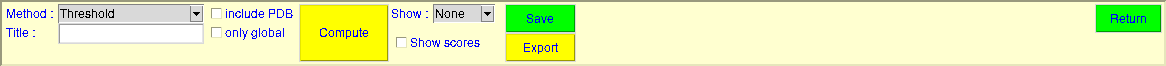
\includegraphics[width=\textwidth, keepaspectratio=true]{conservation_controlpanel.png}
    \caption{The Conservation tool control panel interface.}
\end{figure}

The Control Panel provides the following options:
\begin{itemize}
    \item \textbf{Method}: Selection of the scoring algorithm. Below the separator line, \textbf{GroupSim} predicts specificity-determining positions (section \ref{tool-groupsim}).
    \item \textbf{Title}: An optional label to identify the specific computation.
    \item \textbf{Include PDB}: If enabled, includes PDB sequences in the calculation (disabled by default to avoid redundancy with the corresponding PDB genomic sequences).
    \item \textbf{Only Global}: If checked, group-specific conservation is ignored, focusing only on the entire alignment.
    \item \textbf{Compute}: Launches the conservation analysis.
    \item \textbf{Show}: a dropdown menu to navigate between the computations of the session, listed with their title. Temporary results are named \textit{tmpCons-<Method>\_<n>} (\textit{tmpCons-T<threshold>} for the Threshold method).
    \item \textbf{Show Scores}: check button opening a graphical frame below the alignment that displays the selected conservation scores.
    \item \textbf{Save}: saves the selected result as a new Feature named \textit{Cons-<Method>} (with a \textit{\_<n>} suffix if the name already exists), making it accessible in the main 'Normal' mode. Remember to save the instance (\textit{Overwrite} or \textit{New Instance}) to keep it.
    \item \textbf{Export}: saves the selected result, then writes its scores in a CSV file named \texttt{<alignment file>\_<feature>.csv}: one row per group (\textit{all} for the whole alignment), one column per alignment position.
    \item \textbf{Return}: Exits the tool, close the 'Scores' frame if opened, and returns to the main interface.
\end{itemize}


\subsection{The 3D Viewer Tool}
\label{tool-3dviewer}

The \textbf{3D Viewer} is one of the most powerful tools in Ordalie. While it is not intended to replace dedicated molecular visualization software like VMD or PyMol, it is specifically designed to bridge the gap between sequence features and 3D structural analysis.

\subsubsection{Molecules and Objects}
The viewer is organized around two fundamental concepts:
\begin{itemize}
    \item \textbf{Molecule}: Represents all atoms, residues, and chains associated with a specific structure entry.
    \item \textbf{Object}: A custom-defined selection of elements (entire chains, specific domains, residues, or ligands) belonging to a Molecule.
\end{itemize}

\textit{Note:} Feature mapping is applied exclusively to \textbf{Objects}. By default, Ordalie automatically generates three objects for each chain:
\begin{itemize}
    \item \texttt{AL\_<molecule>\_<chain>}: A stick representation of all atoms.
    \item \texttt{CT\_<molecule>\_<chain>}: A C\textalpha (or phosphate) backbone trace.
    \item \texttt{CA\_<molecule>\_<chain>}: A ribbon (cartoon) representation.
\end{itemize}

\attention{At present, Ordalie does not handle hydrogen atoms.}

\subsubsection{Representation Types}
Multiple styles are available to visualize structural data:
\begin{itemize}
    \item \textbf{Ribbon}: A smoothed path following C\textalpha (amino acids) or P (nucleic acids) atoms.
    \item \textbf{C\textalpha/P Trace}: A simplified line connecting successive C\textalpha or P atoms.
    \item \textbf{CPK}: Space-filling spheres based on Van der Waals (VDW) radii.
    \item \textbf{Pearls}: A simplified view where each residue is represented by a single sphere at its center of mass.
    \item \textbf{Ribbon + Atoms} and \textbf{Ribbon + CPK}: a ribbon with the atoms of the residues drawn as sticks or as spheres.
    \item \textbf{Atoms}: A wireframe (line) representation. Standard residues follow internal topology rules, while other compounds (ligands, modifications) use distance-based bonding, which may vary depending on structure quality.
\end{itemize}

\subsubsection{The 3D Viewer Interface}
The window is divided into five main functional areas (see figure \ref{3dviewerinterface}):
\begin{enumerate}
    \item \textbf{Atom Information} (Top): Displays details about picked atoms.
    \item \textbf{Quick Mapping Panel} (Below information): For rapid feature visualization.
    \item \textbf{Molecular Objects Frame} (Center-left): Lists defined molecules and their objects.
    \item \textbf{3D Window} (Center-right): The main interactive viewport.
    \item \textbf{Actions Panel} (Far right): Toolset for analysis and export.
\end{enumerate}


\begin{figure}[htbp]
\centering
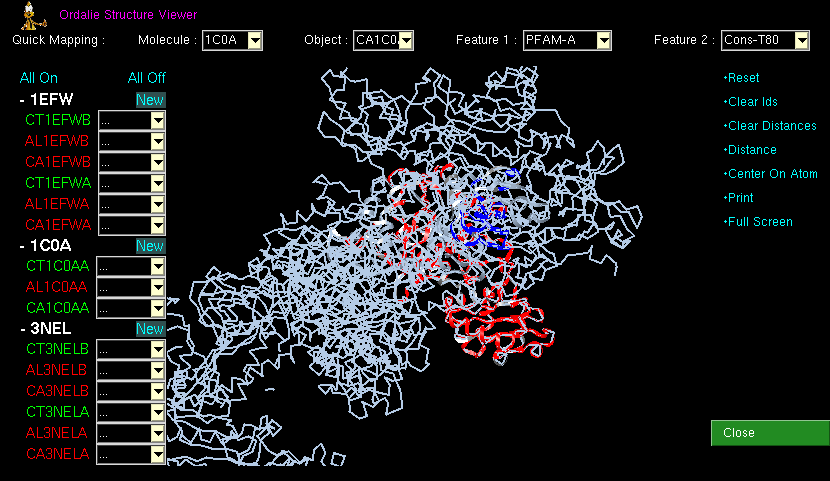
\includegraphics[width=\textwidth, keepaspectratio=true]{window_3D.png}
\caption{The 3D viewer interface}
\label{3dviewerinterface}
\end{figure}


\paragraph{Keyboard Shortcuts}
\begin{itemize}
    \item \textbf{<F1>}: toggles full-screen mode (\textbf{<Escape>} leaves it).
    \item \textbf{<F2>}: Toggles the visibility of all side and top panels.
    \item \textbf{<Ctrl> + <p>}: prints the scene (PNG image).
    \item \textbf{<Ctrl> + <f>} / \textbf{<Ctrl> + <g>}: increases / decreases the depth cueing (fog); \textbf{<Ctrl> + <F1>} switches it on or off.
\end{itemize}

\paragraph{Quick Mapping}
This panel uses four comboboxes to map features onto structures. You can map up to two features simultaneously on a single object. 
The first combobox selects the molecule and the second one an object of this molecule. Choosing an object centres the view on it and, if it was hidden, makes it visible (its name turns \textbf{green} in the Molecular Objects Frame).
\textit{Important:} Features are rendered sequentially (Feature 1 then Feature 2). If Feature 2 covers a larger area (like a PFAM domain) than Feature 1 (like Conservation), Feature 1 might be hidden. In such cases, reverse the order: set PFAM as Feature 1 and Conservation as Feature 2.

\paragraph{Molecular Objects Frame}
This frame manages the hierarchy of structures:
\begin{itemize}
    \item \textbf{Status}: Object names in \textbf{green} are visible; names in \textbf{red} are hidden.
    \item \textbf{All On / All Off}: Switches visibility for every defined object.
    \item \textbf{-/+ <molecule>}: collapses or expands the list of objects of a molecule.
    \item \textbf{New}: creates a new object for the molecule (see section~\ref{chap-objecteditor}).
    \item \textbf{Action menu}: each object has a dropdown menu to \textit{Edit}, \textit{Delete} or \textit{Center} (centre the view on) the object.
\end{itemize}

\paragraph{Interaction in the 3D Window}
Ordalie uses a virtual \textbf{Arcball} (trackball) system for navigation:
\begin{itemize}
    \item \textbf{Rotate}: Drag with mouse \textbf{Button-1} (Left click).
    \item \textbf{Zoom}: Use the \textbf{Mouse Wheel}.
    \item \textbf{Translate (Pan)}: Drag with mouse \textbf{Button-3} (Right click).
    \item \textbf{Identify}: \textbf{<Control-Button-1>} click on an atom to display its label.
\end{itemize}

\paragraph{The Actions Panel}
Key functionalities include:
\begin{itemize}
    \item \textbf{Distance}: calculates the distance between two sequentially picked atoms; \textbf{Clear Distances} removes them.
    \item \textbf{Clear Ids}: removes the labels of picked atoms.
    \item \textbf{Center On Atom}: centers the rotation of the scene on the last picked atom.
    \item \textbf{Print}: exports the current scene as a PNG image.
    \item \textbf{Full Screen}: same as \texttt{<F1>}.
    \item \textbf{Reset}: resets the view and ongoing picking actions.
    \item \textbf{Close}: closes the 3D Viewer.
\end{itemize}

\subsubsection{The Object Editor}
\label{chap-objecteditor}
An object is an ensemble of residues and/or ligands belonging to one or several chains, and displayed in given styles with given colours. The Object Editor can be invoked to create a new object (the 'New' button) or to edit an existing object (\textit{Edit} in the action menu of the object, see the Molecular Objects Frame above).

\begin{figure}[h!]
    \centering
    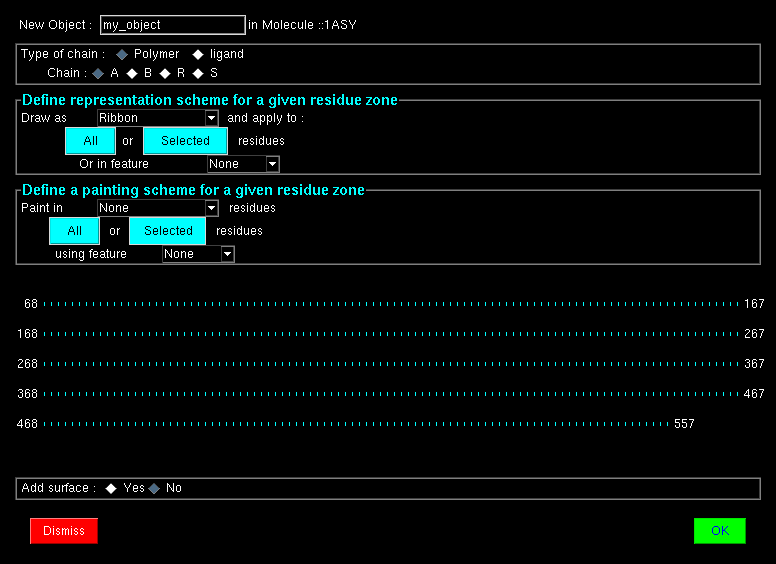
\includegraphics[width=0.75\textwidth, keepaspectratio=true]{3dviewer_create.png}
    \caption{The 3D object creation and edition interface.}
\end{figure}
The name of a new object is entered in the entry box at the top of the interface. Be aware that objects names should be unique. Then 
the creation or edition of an object is an iterative five-step process:
\begin{enumerate}
    \item Select the \textbf{Chain} and components (Polymer residues or Ligands).
    \item Select a \textbf{Representation Type}.
    \item Define the \textbf{Residue Range} for that style.
    \item Select a \textbf{Colour}.
    \item Define the \textbf{Residue Range} for that colour.
\end{enumerate}

This process is iterated until all pieces of the object are set up.

Finally, the molecular surface surrounding the object atoms can be added with the \textbf{Add surface} Yes/No buttons at the bottom of the window. A new object has no surface by default (\textit{No}). When an existing object is edited, these buttons show whether it has a surface, and choosing \textit{No} removes it. Click \textbf{OK} to create the object, or \textbf{Dismiss} to cancel.

\paragraph{Residue Selection Methods}
Three modes of residue selection are available for applying representation types or colors:
\begin{itemize}
    \item \textbf{All}: Applies to the entire chain.
    \item \textbf{Selected}: Applies to residues highlighted in the residue frame (via click-and-drag with Button-1).
    \item \textbf{Feature}: Selects residues based on a predefined sequence feature (e.g., specific domains or conserved sites).
\end{itemize}

The object is then finished by clicking on the 'OK' button. The new object will be added to the object list on the corresponding molecule.



\subsection{The Superposition Tool}
\label{tool-superposition}

One of the key strengths of Ordalie is its ability to map sequence-based features onto 3D protein models. To fully exploit this mapping, it is essential to account for structural differences between proteins. The Superposition tool allows users to align 3D structures based on specific features or user-defined residue ranges. The tool requires at least two structures in the instance; when only one structure is present, the 3D Viewer is opened directly.

\subsubsection{The Superposition Algorithm}
A protein structure may consist of several chains, which can be identical or distinct. Each chain typically comprises an amino acid polymer and various ligands (in Ordalie, water molecules are treated as ligands). 

\attention{While superposition calculations are performed using polymer sequences, the entities physically moved in the 3D space are the entire chains. Applying a superposition to a chain moves all its components, including both the polymer residues AND the ligands.}

The chain superposition process follows three steps:
\begin{enumerate}
    \item \textbf{Zone Selection}: Identification of the structural regions to be used for the alignment (e.g., an entire domain or specific secondary structures).
    \item \textbf{Chain Selection}: Selection of all chains that need to be moved or used as a reference.
    \item \textbf{Reference Selection}: Choosing one chain among the selected ones to act as the fixed reference. All other chains will be aligned onto this stationary target.
\end{enumerate}

The detailed mathematical superposition algorithm is presented in Appendix \ref{app-superposition}.

\subsubsection{Control Panel}

\begin{figure}[htbp]
    \centering
    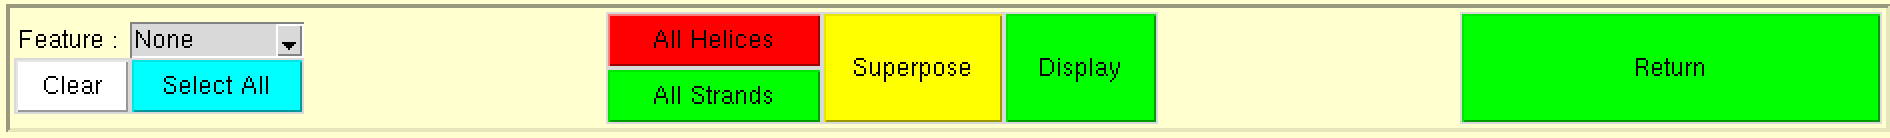
\includegraphics[width=\textwidth, keepaspectratio=true]{superposition_controlpanel.png}
    \caption{The Superposition tool control panel.}
\end{figure}

\paraluc{Selection Tools}
The left part of the panel manages the residues used for the alignment calculation:
\begin{itemize}
    \item \textbf{Features}: Displays the active feature. Users can select specific feature items (\texttt{<Ctrl> + <B1>}) to define the residue range.
    \item \textbf{Clear}: Resets all current residue and sequence selections.
    \item \textbf{Select All}: Selects all residues in the current instance.
    \item \textbf{All Helices}: Selects all helical regions across the sequences.
    \item \textbf{All Strands}: Selects all \textbeta-strands across the sequences.
\end{itemize}

\attention{The 'All Helices' and 'All Strands' options identify the minimal common intersection of secondary structures at each position across all selected sequences.}

\paraluc{Control Tools}
\begin{itemize}
    \item \textbf{Superpose}: Launches the alignment process. This triggers two sequential windows:
    \begin{enumerate}
        \item The \textbf{Chain Selection} window to pick all chains involved.
        \item The \textbf{Reference Chain} window to designate the fixed structure.
    \end{enumerate}
    \item \textbf{Display}: Opens the \textbf{3D Viewer} for visual inspection (see Section \ref{tool-3dviewer}).
    \item \textbf{Return}: Exits the Superposition tool.
\end{itemize}

\subsubsection{Example: Handling a Homo-dimer}
Consider a protein known to be a homo-dimer (an $\alpha_{2}$ quaternary structure). Suppose we have two structures from different organisms, PDB 1abc and 1def, both composed of chains A and B. If the alignment contains only the sequences \texttt{PDB\_1abc\_A} and \texttt{PDB\_1def\_A}:

\paragraph{Scenario 1: Single chain in the instance}
Ordalie identifies the PDB IDs and downloads the full atomic coordinates for both structures (including chains B). However, if you superpose \texttt{PDB\_1def\_A} onto \texttt{PDB\_1abc\_A}, only the atoms of 1def Chain A will be aligned. In the 3D Viewer, the 1abc dimer remains intact, but for 1def, Chain A will be correctly placed while Chain B will remain in its original coordinate space, effectively "breaking" the 1def dimer symmetry.

\paragraph{Scenario 2: Moving a complete multimer}
Ordalie does not automatically infer multimeric states; the user must define the chains of interest.

\idee{To manipulate a multimer, all sequences corresponding to the chains of both the reference AND the target structure must be present in the alignment.}

If the alignment contains \texttt{PDB\_1abc\_A}, \texttt{PDB\_1abc\_B}, \texttt{PDB\_1def\_A}, and \texttt{PDB\_1def\_B}, you can superpose the dimers in two steps:
\begin{enumerate}
    \item Superpose \texttt{PDB\_1def\_A} onto \texttt{PDB\_1abc\_A}.
    \item Superpose \texttt{PDB\_1def\_B} onto \texttt{PDB\_1abc\_B}.
\end{enumerate}
This ensures the entire biological assembly is correctly aligned in the 3D space.


\subsection{The Features Editor Tool}
\label{tool-feateditor}

This tool is dedicated to feature management, including creation, deletion, and edition of sequence characteristics.

\subsubsection{Control Panel}
The Control panel of the \textbf{Features Editor} provides quick access to global actions.

\begin{figure}[h!]
    \centering
    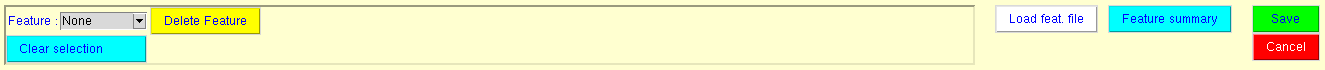
\includegraphics[width=\textwidth, keepaspectratio=true]{feateditor_controlpanel.png}
    \caption{The Control panel of the Feature Editor tool}
\end{figure}

The panel includes the following options (from left to right):
\begin{itemize}
    \item \textbf{Features:} Displays the currently selected feature. The user can select a specific feature item as a residue range.
    \item \textbf{Clear Selection:} Resets all residue ranges and sequences previously selected.
    \item \textbf{Delete Feature:} Permanently removes the current feature across all sequences.
    \item \textbf{Load Feat. File:} Imports a file containing user-defined features (see Appendix \ref{chap-featurefile} for format details).
    \item \textbf{Features Summary:} Launches the summary tool for an overview of all features within the instance (see section \ref{tool-featsummary}).
    \item \textbf{Save:} Commits changes and returns to 'Normal' mode. Saved features are marked as changes of the instance: use \textit{Overwrite} or \textit{New Instance} to keep them.
    \item \textbf{Cancel:} discards changes, restores original features, and returns to 'Normal' mode.
\end{itemize}

\subsubsection{Notation and Actions}
It is essential to distinguish between a \textbf{Feature} and a \textbf{Feature Item}:
\begin{itemize}
    \item \textbf{Feature:} A general set of items representing a specific sequence characteristic (e.g., "Alpha Helix").
    \item \textbf{Feature Item (or Item):} A single occurrence of a Feature at a specific position for a specific sequence.
\end{itemize}

\subsubsection{Contextual Menu}
Unlike other tools, the Feature Editor allows direct interaction within the instance window via a right-click contextual menu.

\attention{In this tool, the behavior of \texttt{<Button-1>} (Left Click) is modified by modifier keys:
    \begin{itemize}
        \item \texttt{<Button-1>} alone: Applies action to the sequence under the pointer.
        \item \texttt{<Control + B1>}: Applies action to the entire group containing the sequence.
        \item \texttt{<Shift + B1>}: Applies action to all sequences in the instance.
    \end{itemize}
}

\paragraph{Select Item}
Selects the Item directly under the mouse pointer. The scope (sequence, group, or all) depends on the modifier keys mentioned above. If <Control> is pressed with <Button-1> then the item present in the sequences of the current group will be selected. If <Shift> is pressed then the item present in all sequences of the instance will be selected.

\paragraph{Select All Items}
Selects all Items of a sequence, a group, or the whole instance depending on the modifier key. 

\idee{Selecting all Items for all sequences effectively selects the entire Feature. If deleted, the Feature itself is removed from the project.}

\paragraph{Select Region}
Define a residue range by clicking and dragging \texttt{<Button-1>}. This region can be used to define a new Item. The scope follows the standard \texttt{Control/Shift} modifiers.

\paragraph{Clear Selection}
Clears all active selections.

\subsubsection{Edition Options}
After selecting Items or a region, the following options become available in the menu:

\paragraph{Edit Item}
Modifies properties of existing Items. If multiple Items are selected, some properties may be locked unless they refer to a single zone:\textbf{Residue range} (Only editable for single-zone selections), \textbf{Item Colour}, \textbf{Score}, and \textbf{Note}.

\paragraph{Define New...}
Opens a configuration window:
\begin{itemize}
    \item If the \textbf{Feature Name} matches an existing one, the item is added to that feature.
    \item If the name is new, a new Feature is created.
    \item Users must assign a \textbf{Colour}; \textbf{Score} and \textbf{Note} are optional.
    \item Spaces in the feature name are replaced by underscores.
    \item The colour is a colour name or a \texttt{\#RRGGBB} value; the \textit{More Colors} entry of the colour list opens a colour chooser. The score must be a real number (default 0.0).
\end{itemize}

\paragraph{Delete Selected Items}
Removes the selected items. Deleting all items of a feature will result in the deletion of the feature itself.

\paragraph{Propagate Items (Group/All)}
\textbf{Propagate Item to this group} copies the selected Item to all sequences of its group, while \textbf{Propagate Item to all} copies it to every sequence of the instance. Only one Item must be selected. Sequences already having the same Item are skipped, and an Item in local coordinates that falls on a gap of a target sequence is stored in global coordinates.


\subsection{The Features Summary}
\label{tool-featsummary}

The \textbf{Features Summary} tool allows the simultaneous rendering of multiple selected sequences and their associated features on a single page. Unlike the \textit{Instance Overview}, sequences in this view maintain their appearance as seen in the main alignment window.

\begin{figure}[h!]
    \centering
    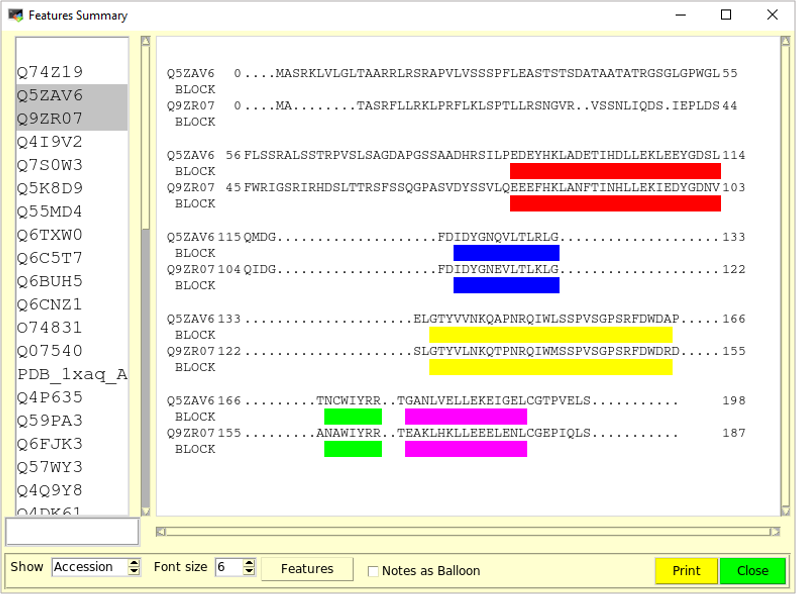
\includegraphics[width=\textwidth, keepaspectratio=true]{featsummary_window.png}
    \caption{The Features Summary window, showing the Drawing Area (top) and the Control Panel (bottom).}
\end{figure}

\subsubsection{Drawing Area}
The upper portion of the window consists of a listbox for sequence selection and a main drawing area.
Clicking a sequence name in the listbox toggles its selection. Multiple sequences can be selected by holding the \texttt{<Control>} key while clicking. For each selected sequence, the display includes:
    \begin{itemize}
        \item The \textbf{Sequence ID} on the left.
        \item The \textbf{Start and End positions} of the residues for the current line.
        \item The \textbf{Amino acid sequence} as it appears in the alignment.
    \end{itemize}
When a feature is active, a dedicated line appears below the sequence. The feature name is displayed under the sequence ID, and colored rectangles mark the positions where the feature is present. The entire view can be panned by clicking and dragging with \texttt{<Button-1>}. The mouse wheel scrolls the drawing vertically, and \texttt{<Ctrl> + <Mouse-wheel>} horizontally. A double click on a feature rectangle centres the main alignment window on this feature.

\subsubsection{Control Panel}
Located below the drawing area, the Control Panel provides several configuration options:

\begin{description}
    \item[ID Type Selector (Spinbox):] Choose how sequences are referenced (Sequence Name, Accession Number, or Bank ID). This change updates both the listbox and the drawing area.
    \item[Font Size Selector:] Adjusts the text scale for better readability.
    \item[Features Selector:] A list of checkboxes allowing the user to overlay any number of features onto the sequences.
    \item[Notes as Balloon:] When enabled, the notes attached to a feature appear as a tooltip (balloon) when hovering over the feature with the mouse.
    \item[Print:] Prompts for a filename to export the current drawing area as a \textbf{PNG image}.
    \item[Close:] Exits the tool and closes the window.
\end{description}


\subsection{The Annotation Tool}
\label{tool-annotate}

This tool allows users to add, modify, and remove "memo tags" anywhere on the instance. These annotations can be toggled on or off at any time using the \textbf{Annotations} button located on the instance bar. The tool can be started from the main window only (leave the other tools first). While it is active, all the annotations of the instance are displayed.

A memo tag is defined by three main characteristics: its position and size, its color, and its attached text note. These tags are particularly useful for marking zones of interest, such as conserved regions or areas requiring manual re-alignment. Furthermore, color-coding can serve as a classification system—for example, using pink for structural annotations and cyan for sequence features.

\subsubsection{Control Panel}
The Control Panel is designed for straightforward management of visibility and tool states. From left to right, it includes:
The \textbf{Show annotations colored in} combobox (\textit{None}, \textit{All}, or one of the colours in use) filters the display, while \textbf{Show All} and \textbf{Hide All} show or hide all the annotations. \textbf{Return} keeps the changes (new, edited and deleted annotations) as changes of the instance and leaves the tool: use \textit{Overwrite} or \textit{New Instance} to save them (they are also saved when switching instance, if you choose so, or when saving the file); \textbf{Dismiss} leaves the tool and forgets the changes made since it was started.

\subsubsection{Keyboard Bindings}
Annotation creation and editing are primarily mouse-driven. The interaction logic is summarized in Table \ref{table-keysanno}.

\begin{table}[h!]
\centering
\begin{tabular}{|l|p{10cm}|}
\hline
\textbf{Keys} & \textbf{Action} \\
\hline
\hline
\texttt{<Button-1>} & Select the origin of a new annotation. \\
\texttt{<Button-1> dragging} & Define the area of the current annotation. \\
\texttt{<Button-1> release} & Finalize the annotation zone definition. \\
\hline
\texttt{<Control> + <Button-1>} & Delete the annotation below the mouse pointer. \\
\hline
\texttt{<Shift> + <Button-1>} & Edit the existing annotation below the mouse pointer. \\
\hline
\end{tabular}
\caption{Keys combination for annotation management}
\label{table-keysanno}
\end{table}

Upon releasing the mouse button after defining a zone, a window appears next to the pointer to choose the annotation colour and enter its text (\texttt{<Ctrl> + <Return>}: OK, \texttt{<Escape>}: Cancel). The same window is used to edit an annotation. Separator lines are not part of a zone. Finally, clicking \textbf{Return} ensures all changes are committed.

Annotations are attached to the sequences, not to display lines: they follow the sequences when the instance is reordered. They are saved in ORD files, and exported in Macsim/XML files as a feature named \textit{SnapAnnotation}, read back as annotations. In the main window, the \textbf{Annotations} button of the instance bar shows or hides the annotations of the current instance (they are updated when another instance is selected), and the text of an annotation appears in a balloon when the mouse is over it.


\subsection{Barcode}
\label{tool-barcode}

The \textbf{Barcode} tool provides an alternative schematic representation of an instance, offering a condensed bird's-eye view of the alignment. A typical example of this visualization is shown in Figure \ref{fig-barcode}.

\begin{figure}[h!]
    \centering
    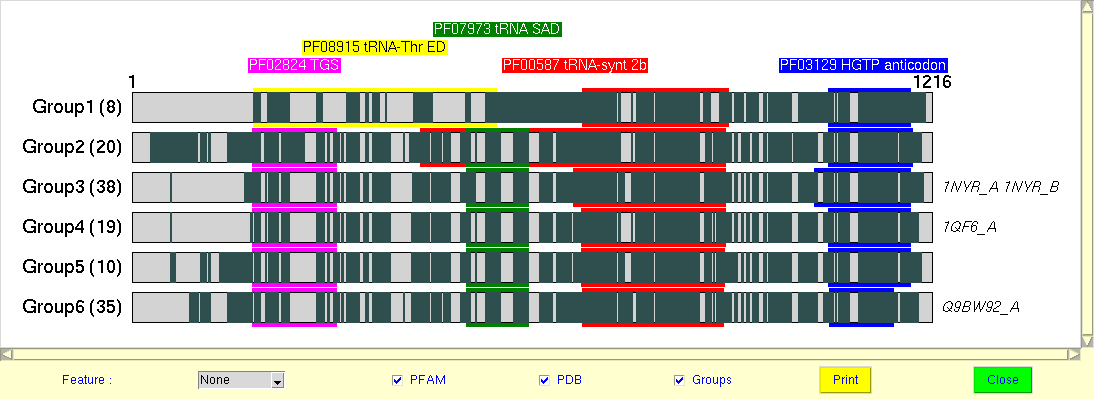
\includegraphics[width=\textwidth, keepaspectratio=true]{barcode.png}
    \caption{The Barcode window.}
    \label{fig-barcode}
\end{figure}

The upper frame of the tool contains the drawing area. A lane is drawn for each group of sequences of the instance, labelled with the group name and its number of sequences (or a single lane, \textit{all}, when the instance is not clustered or when \textbf{Groups} is unchecked). In each lane, the alignment columns where at least 10\% of the sequences of the group have a residue are drawn in dark grey, the other ones in light grey, giving a "barcode" signature of the group. This allows a rapid comparison of the insertion/deletion patterns between groups. The drawing can be moved by dragging it with \texttt{<Button-1>}.

\subsubsection{Control Panel}
\begin{itemize}
  \item \textbf{Feature}: draws the items of the chosen feature (for the sequences of each group) in the lower third of the lanes.
  \item \textbf{PFAM}: draws the PFAM domains as coloured boxes around the lanes of the groups where they are present, with the domain identifier and name above the lanes.
  \item \textbf{PDB}: writes, at the right of each lane, the PDB structures belonging to the group.
  \item \textbf{Groups}: one lane per group (checked, default) or one lane for the whole instance.
  \item \textbf{Print}: exports the whole drawing as a PNG image.
  \item \textbf{Close}: closes the Barcode window.
\end{itemize}
The Barcode shows the instance displayed when it was opened: select the \texttt{Barcode} menu item again to update it after a change of instance.


\newpage
\section{Menus Description}
\label{chap-menus}
This chapter describes all the Ordalie menus. Only the entries which have not been already explained in the 'Tools' section \ref{chap-tools} will be described in details here.

\subsection{The File Menu}
\subsubsection{Open}
Opens an alignment file. Several file formats are recognized:
\begin{itemize}
\item TFA (Fasta) file format, extensions \texttt{.tfa}, \texttt{.fa}, \texttt{.fasta}, \texttt{.tfasta}.
\item MSF (Multiple Sequence File, GCG Wisconsin Package) format, extension .msf.
\item Macsim/XML format. The Macsim format is an XML file output of the MACSIMS program or server (see \cite{soft:macsims} and \url{http://www.lbgi.fr/~julie/MACSIMS/} for details). Accepted extensions are .xml, .macsim, .macsims.
\item ALN (ClustalW) file format \cite{soft:clustalw}, extensions \texttt{.aln}, \texttt{.clustal}.
\item RSF file format (Rich Sequence File), as output by the SeqLab program \cite{soft:seqlab}, extension .rsf.
\item ORD (Ordalie) file, Ordalie specific file format, extension \texttt{.ord}.
\end{itemize}

The \texttt{Open ...} item is a cascade menu: select the format of the file to be read, then choose the file. The chosen format is trusted and is not checked against the file content. 

\subsubsection{Save}
Saves the alignment in the current file format with the current file name (\texttt{<Ctrl> + <s>}). The first time, the user is prompted for a file name; subsequent calls to ``Save'' use the defined name and file format. Unsaved changes of the current instance are first stored in the instance (in a new instance named \textit{Modified alignment} if the current one is the read-only original alignment). The ORD format saves all the instances, sequence data, structures and session state; the other formats save the sequences of the current instance only.

\subsubsection{Save As ...}
Ask for a file format and a file name to save the current instance. If there are selected sequences, the user is asked to save all sequences or the selected ones. Available formats are TFA, MSF, Macsim/XML, ALN (ClustalW) and ORD; RSF files can be read but not written. A warning is displayed if the file extension does not match the chosen format.

\subsubsection{Save Window As}
Save only the visible part of the instance in the specified file format and file name. Available formats are TFA, MSF and ALN.

\subsubsection{Close}
Close all instances and all dependencies (Overview, 3D Viewer... ), and set Ordalie ready to load a new file.

\subsubsection{Print}
When the 'Print' option is invoked, a 'Setup' properties window will pop up. Several printing parameters can be set:
\begin{itemize}
\item image format : actual choices are PostScript, JPEG and PNG.
\item Paper size : A4, A3, US letter, or \textit{Unlimited} (the whole alignment on a single page).
\item Paper orientation : Landscape or Portrait
\item Font size and weight : the font used to print alignments is always Courier New. By default, the font size is the same as the one used in the main Ordalie window. It can be changed from 6 to 16 by steps of 2 pts, and the weight of the font can be 'normal' or 'bold'.
\item Print Area : By default, the whole alignment is printed. It is possible to print only the current window or the selected sequences can be printed too.
\item Ruler : if desired, a ruler can be printed at the bottom of every page.
\item Residue numbering : if desired, the residue numbering inside the sequence can be printed on every page for every sequences.
\end{itemize}
The \textbf{Defauts} button restores the default parameters.

\subsubsection{Quit Ordalie}
Quits Ordalie (\texttt{<Alt> + <F4>}).

\subsection{The Edit Menu}
\subsubsection{Cut}
Cut the selected sequences.

\subsubsection{Copy}
Copy the selected sequences into the memory buffer.

\subsubsection{Paste}
This command pastes the sequences currently stored in the clipboard. Sequences are inserted immediately following the currently selected sequence. If no sequence is selected, no sequences are pasted. When pasting sequences that already exist in the instance, their names will be automatically suffixed with \texttt{\_\_<n>}, where \texttt{<n>} denotes the copy number.

\subsubsection{Preferences}

Open the \textit{Preferences} panel to access the default internal parameters of Ordalie. 

\begin{figure}[htbp]
\centering
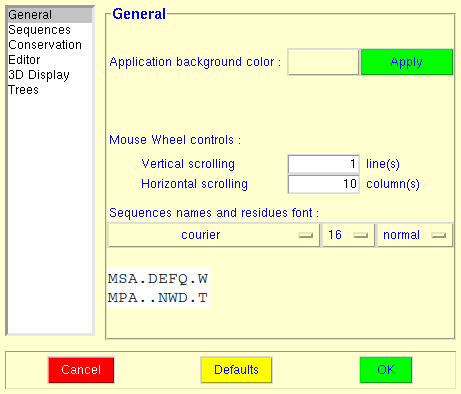
\includegraphics[width=\textwidth, keepaspectratio=true]{preferences.png}
\caption{The Preferences panel.}
\label{preferences}
\end{figure}

Figure~\ref{preferences} shows the \textit{Preferences} panel. Clicking an item in the list box on the left displays the corresponding settings. Preferences are applied to the current display when \textbf{OK} is pressed, and saved in the file \texttt{\$HOME/.ordalierc} (\texttt{ordalierc.def} in the \texttt{APPDATA} folder under Windows), so that they are restored at the next start-up. \textbf{Cancel} discards the changes, and the \textbf{Defaults} button restores the default values of the page currently shown only. Closing the window is equivalent to \textbf{Cancel}.

\begin{itemize}
\item \textbf{General}
\begin{itemize}
\item \textbf{Application background:} Click the coloured button to choose the application background colour. The \textit{Apply} button shows the new colour at once; it is kept with \textbf{OK} and discarded with \textbf{Cancel}.
\item \textbf{Mouse wheel controls:} Defines the number of lines or columns moved for each mouse wheel increment.
\item \textbf{Sequence names and residues font:} Menu buttons allow selection of font family, size, and weight (normal or bold). Changes are previewed immediately in the main window.
\end{itemize}

\item \textbf{Sequences}
\begin{itemize}
\item \textbf{Remove bank prefix when loading sequences:} Sequence names may be prefixed by their database identifier. By default, Ordalie removes this prefix.
\item \textbf{Bank prefixes:} Ordalie recognizes the following prefixes by default (case-insensitive): SPT, SW, SP, TR, UNP, REF, GB, DBJ, ENA, ENS, PDB, VARSPLIC, UniRef90, UniRef100, PQS. A new prefix can be typed in the text field and added with \textit{Add} (or \texttt{<Return>}); a prefix selected in the list can be removed with \textit{Remove selected prefix}.
\item \textbf{Life domain colors:} Click the \textit{Eukaryota}, \textit{Archaea}, \textit{Bacteria}, or \textit{Viruses} buttons to change the associated colors using a color palette.
\end{itemize}

\item \textbf{Conservation}
\begin{itemize}
\item \textbf{Conservation type colors:} Defines foreground and background colors for the three conservation levels used in Ordalie. Changes apply to the next conservation computations.
\item \textbf{Threshold:} Threshold (0-100\%, default 80\%) above which a column is considered conserved by the \textit{Threshold} method.
\item \textbf{Use similarity:} Includes physicochemical similarity when computing conservation. Default is \textit{Yes}.
\end{itemize}

\item \textbf{Editor}
\begin{itemize}
\item \textbf{Lock sequences at start-up:} By default, only gaps can be added or removed. Selecting \textit{Yes} allows amino acid insertion or deletion in the editor.
\item \textbf{Residue mapping colors:} Defines how residues are displayed in the editor. The default scheme is based on the SeqLab editor \cite{soft:seqlab}. The \textit{Colorblind Mapping} button selects a colour scheme suited to colour-blind users, and \textit{Default Mapping} restores the original colours. The residue colours are kept separately for protein and nucleic acid alignments.
\end{itemize}

\item \textbf{3D Display}
\begin{itemize}
\item \textbf{Default ribbon color:} Color used for ribbon representation when no feature is applied.
\item \textbf{Precompute surface:} Determines whether the solvent-accessible surface is computed when creating a new object. Default is \textit{No}.
\item \textbf{Color ramps:} colours used by \texttt{Structures} $\rightarrow$ \texttt{Color Sec. Str by identity}. Clicking a button changes the corresponding colour.
\end{itemize}

\item \textbf{Trees}
\begin{itemize}
\item \textbf{Gap removal:} Selects the gap removal strategy (see Section~\ref{control-tree}). Default is \textit{Pairwise}.
\item \textbf{Type of tree:} Dendrogram (default) or Circular (radial) tree.
\item \textbf{Tree font:} Defines size and weight (normal or bold) for tree labels.
\item \textbf{Bootstrap:} Enables tree bootstrapping. Default is \textit{No}.
\end{itemize}
\end{itemize}


\subsection{The View Menu}

\subsubsection{Bigger Font}
Increases the font size for the sequence display. The default font type and size for Ordalie can be configured via \texttt{Edit} $\rightarrow$ \texttt{Preferences} under the \textbf{General} tab.

\subsubsection{Smaller Font}
Decreases the font size for the sequence display.

\subsubsection{View Log}
\label{viewlog}
Most of Ordalie's operations and computations are recorded in a log. Selecting this item opens a sub-menu to display the log either in a console window (\textit{in Console}) or in a web browser as an HTML document (\textit{in browser}). The console window has buttons to save its content as a text file, to clear it and to close it.

\subsubsection{Save Log File}
Exports the entire Ordalie log to a file. A sub-menu allows the user to choose between HTML and Text formats. The output file name is derived from the root name of the original alignment file, appended with the corresponding extension (\texttt{.txt} or \texttt{.html}).

In the HTML log (saved, or displayed with \textit{View Log}, then \textit{in browser}), each table is followed by a \textbf{Download CSV} button that saves this table as a CSV file, named after the table title. The script doing it is embedded in the HTML file, so the file can be moved or sent on its own. As for any web download, the browser chooses where the file is written: by default in the user's \textit{Downloads} folder (on macOS, Safari uses the location set in the \textit{Safari} menu, \textit{Settings}, \textit{General} tab, \textit{File download location}; some browsers ask for a location instead). Fields containing commas, double quotes or line breaks are quoted.

\subsubsection{Toggle Full Screen}
Toggles the main window between its current size and full-screen mode. This action can also be triggered by pressing \texttt{<Ctrl> + <F1>}.

\subsubsection{Show/Hide Icon Bar}
Displays or hides the shortcut icon bar. Hiding this bar is useful when maximum vertical space is required, such as during intensive alignment editing.

\subsubsection{Show/Hide Scores}
Toggles the visibility of the scores panel. When a conservation score is active (enabled via the Features buttons or the \textbf{Conservation} tool), the global and group-specific scores for each column are plotted. By default, the scores panel is hidden.

\subsubsection{Show/Hide Features}
Toggles the visibility of the Features panel. This is useful for maximizing the alignment display area during manual editing.

\subsubsection{Show/Hide Phylum}
If taxonomic information (Life Domain) is available for the sequences, the sequence names are color-coded accordingly (light backgrounds): \textbf{Eukaryota} in pink, \textbf{Archaea} in light blue, \textbf{Bacteria} in light yellow, and \textbf{Viruses} in black (white text). These default colors can be customized in the \textbf{Preferences} panel. Phylum colouring and group colouring are mutually exclusive: activating one deactivates the other.

\subsubsection{Show/Hide Group Colors}
Applies color-coding to sequences based on their assigned groups.

\subsubsection{Show/Hide Secondary Structures}
If secondary structure information is available, this option displays or hides \textalpha-helices (red), \textbeta-strands (green), turns (cyan) and $3_{10}$ helices (magenta).


\subsection{The Sequences Menu}

\subsubsection{Names as}
In Ordalie, there are several ways to display sequence names:
\begin{itemize}
    \item \textbf{Sequence Name}: A user-defined name.
    \item \textbf{Accession Number}: The unique identifier from the source database.
    \item \textbf{Database ID}: The database entry identifier.
    \item \textbf{Full Organism Name}: The complete scientific name (if available).
    \item \textbf{Genus.Species Abbreviation}: A shortened version of the organism name (if available), made of the first four letters of the genus and of the species. For example, \textit{Homo sapiens} becomes \textit{Homo.sapi} and \textit{Saccharomyces cerevisiae} becomes \textit{Sacc.cere}.
\end{itemize}

By default, the \textbf{Sequence Name} is displayed. The chosen type of name is kept when another instance is selected and in the Editor. When the information is not available for a sequence (for example the organism of a sequence read from a FASTA file), its sequence name is displayed instead. PDB sequences always keep their name. The names pane is widened to fit the longest name, up to twice its default width; the complete information on a sequence is shown with \texttt{<B3>} on its name.

In Macsims/XML and Ordalie file formats, the Sequence Name, Accession Number, Bank ID and organism are explicitly given for each sequence. For all other formats, where only one ID per sequence is typically provided, this identifier will be used as the Sequence Name, Accession Number, and Bank ID simultaneously.

\subsubsection{Identity Tool}
Launches the Identity tool; for further details, see Section \ref{tool-identity}.

\subsubsection{Search Motif}
Launches the Search Motif tool; for further details, see Section \ref{tool-motif}.

\subsubsection{Retrieve Sequences Information}
\label{tool-inforetrieve}
This command retrieves up-to-date information for specific sequences by querying their original databases. Upon invocation, a dialog box appears asking whether to process all sequences or only the selected ones. Once confirmed, Ordalie queries the corresponding databases to fetch the latest metadata. 

If any amino acid sequences have been updated in the database, they will be automatically realigned with the existing sequences using the MAFFT program. After completion, a summary window displays the number of updates performed for Accession, Phylum, Taxa ID, Organism, Description, and the amino acid sequence itself. Below the summary table, the ``Show details...'' button opens a web page providing a detailed log of the changes for each sequence.

\subsubsection{Edit Sequence Information}
\label{tool-editinfoseq}
Opens the Sequence Information window. The dropdown menu at the top selects the sequence (by default the first selected sequence, or the first sequence of the instance). The left part shows the fields that can be edited: Sequence Name, Accession, Bank Id, E.C. number, Description, Organism, Life domain (chosen among Eukaryota, Archaea, Bacteria and Viruses), Taxa Id and Lineage. The right part gives the physico-chemical properties (molecular weight, length, hydrophobicity, isoelectric point) and the amino acid composition of the sequence, of its group and of the whole alignment.

Changes are checked and recorded when another sequence is selected or when the window is closed (\textbf{Close} button or window close box): the Sequence Name must be unique and without spaces, the E.C. number must be made of 4 fields (e.g.\ 6.1.1.12 or 6.1.-.-), and the Taxa Id must be an integer; otherwise a warning is displayed and the field is not changed. The names displayed in the main window and the life domain colours (main window and trees) are updated, and the changes are saved with the instance in ORD files.

\subsubsection{Add Feature from File}
Opens a file dialog to import a feature file. Once loaded, these features are immediately available within Ordalie. The supported feature file format is described in Appendix \ref{chap-featurefile}.

\subsubsection{Export Features to File}

This function allows exporting features associated with a selected set of sequences into a feature file (see \ref{chap-featurefile}).

\begin{figure}[htbp]
\centering
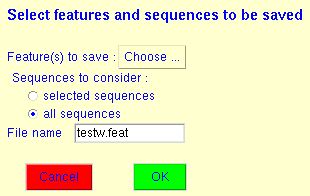
\includegraphics[width=0.5\textwidth, keepaspectratio=true]{window_writefeature.png}
\caption{The Export Features window}
\label{exportfeature}
\end{figure}

Figure \ref{exportfeature} shows the ``Export Features'' window. 

Clicking the \textit{Features} menu button displays the list of available features as a set of checkboxes. The user can select one or more features to export.

The sequences from which the features are extracted can be either all sequences or only the currently selected ones.

Finally, the user must specify the name of the output file. By default, the output file is named after the alignment file with the \texttt{.feat} extension.

\subsubsection{Features Editor}
Launches the Features Editor tool; see Section \ref{tool-feateditor}.

\subsubsection{Features Summary}
Launches the Feature Summary tool; see Section \ref{tool-featsummary}.

\subsubsection{Add Sequences to Instance}
This item opens a menu for adding sequences from databases or local files. This command is not available while the Editor is active.
\begin{itemize}
    \item \textbf{From Database}: Ordalie downloads sequences from UniProt or RefSeq based on a user-provided list of accessions. 
    \item \textbf{From File}: The user provides a sequence file in TFA, MSF, or ALN format for Ordalie to parse.
\end{itemize}

The sequences are then added to the current instance.

A dedicated window appears based on the selection to collect the necessary parameters. Figure \ref{windowaddseq} illustrates the interface for adding sequences from a database.

\begin{figure}[h!]
    \centering
    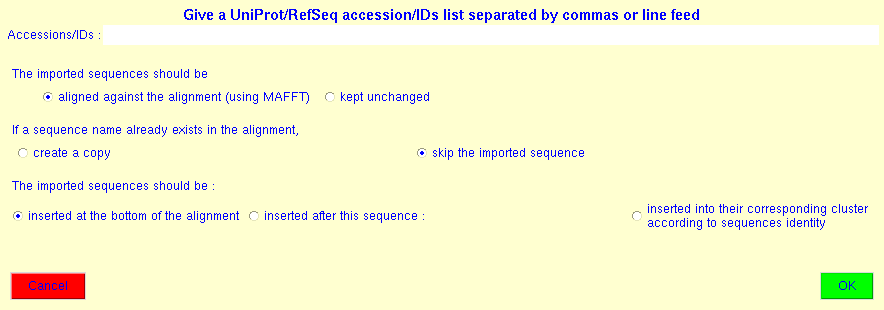
\includegraphics[width=0.5\textwidth, keepaspectratio=true]{window_addseqs_db.png}
    \caption{The interface for adding sequences from a database.}
    \label{windowaddseq}
\end{figure}

After specifying the source, the user should define the following settings:
\begin{itemize}
    \item \textbf{Alignment}: Choose whether the added sequences should be automatically aligned using MAFFT against the existing instance sequences.
    \item \textbf{Duplicates}: Choose whether to discard duplicate sequences or create copies. In the case of duplicates, the new sequence names will be suffixed with \texttt{\_\_<n>}, where \texttt{<n>} represents the copy number.
    \item \textbf{Insertion Point}: Specify whether to append sequences at the bottom of the instance, insert them immediately after a specific sequence (selected via a dropdown menu), or cluster them based on sequence identity (available only if the sequences are being aligned).
\end{itemize}

Once the sequences are added, feature positions are recomputed if necessary. Basic sequence characteristics (isoelectric point, molecular weight, identity, composition, etc.) are then calculated for the new entries and recorded in the log.

\subsubsection{Add structures to Instance}
A structure can be added by specifying a PDB ID (for automatic download from the RCSB database), a UniProt accession to download the corresponding AlphaFold structure if it exists in the EMBL/EBI AlphaFold database, or by providing a local structure file either in PDB or CIF (.cif, .mmcif) formats. The user then chooses which chain(s) to consider: a given chain, the chain automatically selected by Ordalie, or all chains.

\subsection{The Alignment Menu}
\subsubsection{Editor}
Launches the Alignment Editor tool; see Section \ref{tool-editor}.

\subsubsection{Re-Align Sequences}
Re-aligns the selected sequences using the MAFFT program \cite{soft:mafft, soft:mafft2, soft:mafft3, soft:mafft4}. The selected sequences are first degapped and then re-aligned against the remaining sequences. The re-aligned sequences maintain their original vertical positions within the instance.

\subsubsection{Clustering}
Launches the Clustering tool; see Section \ref{tool-clustering}.

\subsubsection{Add Separator}
In Ordalie, a ``separator'' is a blank line inserted between sequences. Sequences separated by these lines constitute a distinct group or cluster. Adding separators allows users to define their own custom clusters. This command inserts a blank separator line immediately below the selected sequence. Note that exactly one sequence must be selected for this operation.

\subsubsection{Remove Separator}
Removes the separator located immediately below the selected sequence. Note that exactly one sequence must be selected.

\subsubsection{Remove All Separators}
Removes all separators and clears all sequence selections, resulting in an unclustered instance.

\subsubsection{Overview}
Opens a new Overview window for the current instance; see the ``Instance Overview'' in Section \ref{tool-overview}.

\subsubsection{Conservation}
Launches the Conservation computation tool; see Section \ref{tool-conservation}.

\subsubsection{Tree Building}
Launches the Phylogenetic Tree tool; see Section \ref{tool-tree}.

\subsubsection{Annotate Instance}
Launches the Annotation tool; see Section \ref{tool-annotate}.

\subsubsection{Barcode}
Launches the Barcode tool; see Section \ref{tool-barcode}.

\subsubsection{Toggle Physicochemical Coloring}
Toggles residue coloring using the same mapping as in the \textbf{Editor}. The residue color scheme can be customized in \texttt{Edit} $\rightarrow$ \texttt{Preferences} under the \textbf{Editor} tab.


\subsection{The Structures Menu}

\subsubsection{Superpose Structures}
Launches the \textbf{Superposition} tool, provided that multiple PDB structures are available in the current instance; see Section \ref{tool-superposition}.

\subsubsection{Display Structures}
Launches the \textbf{3D Viewer} tool; see Section \ref{tool-3dviewer}.

\subsubsection{Color Secondary Structures by Identity}
This tool (``Color Sec. Str. by Identity'' in structure menu) allows for the coloring of secondary structures based on their sequence identity levels within the instance. Upon invocation, a dialog box appears with the following configuration options:
\begin{itemize}
    \item \textbf{Similarity Computation}: Calculate similarities using either the average secondary structure limits or a specific reference sequence.
    \item \textbf{Color Gradient}: Select between a grayscale or a multi-color gradient.
    \item \textbf{Gradient Scale}: Define the limits from the minimum to maximum identity, or across a fixed 0\% to 100\% range.
    \item \textbf{B-factor Assignment}: Choose whether to map the identity scores to the B-factor column of the PDB file.
\end{itemize}
This tool only applies to ribbon representation.
\subsubsection{Save PDB}
Since 3D structures may be modified (e.g., coordinates transformed) using the \textbf{Superposition} tool, this option allows the user to save any 3D structure present in the instance to a file. This is particularly useful for exporting superposed structures to more advanced molecular rendering software.

When selected, a window prompts the user to define the export parameters:
\begin{itemize}
    \item Select the target molecule.
    \item Select either all chains or a specific chain.
    \item Select all residues or a specific residue range.
\end{itemize}

To complete the process, the user will be prompted to specify the output PDB filename.


\subsection{The Help Menu}

\subsubsection{About Ordalie}
This menu item opens a window providing essential information about Ordalie, including the current version number and the link to the official Ordalie home page.

\subsubsection{Local Documentation}
Opens this manual (HTML version) in the built-in hv3 HTML viewer.

\subsubsection{Online Documentation}
Launches the Ordalie documentation in a web browser, redirecting to the official Ordalie website.


\newpage
\section{Appendix}
\subsection{The Ordalie database scheme}
\label{chap-schemedb}
The core of Ordalie is built around an in-memory SQLite database \cite{soft:sqlite} whose schema is given in figure \ref{ordalie-db-scheme}.

\begin{figure}[htbp]
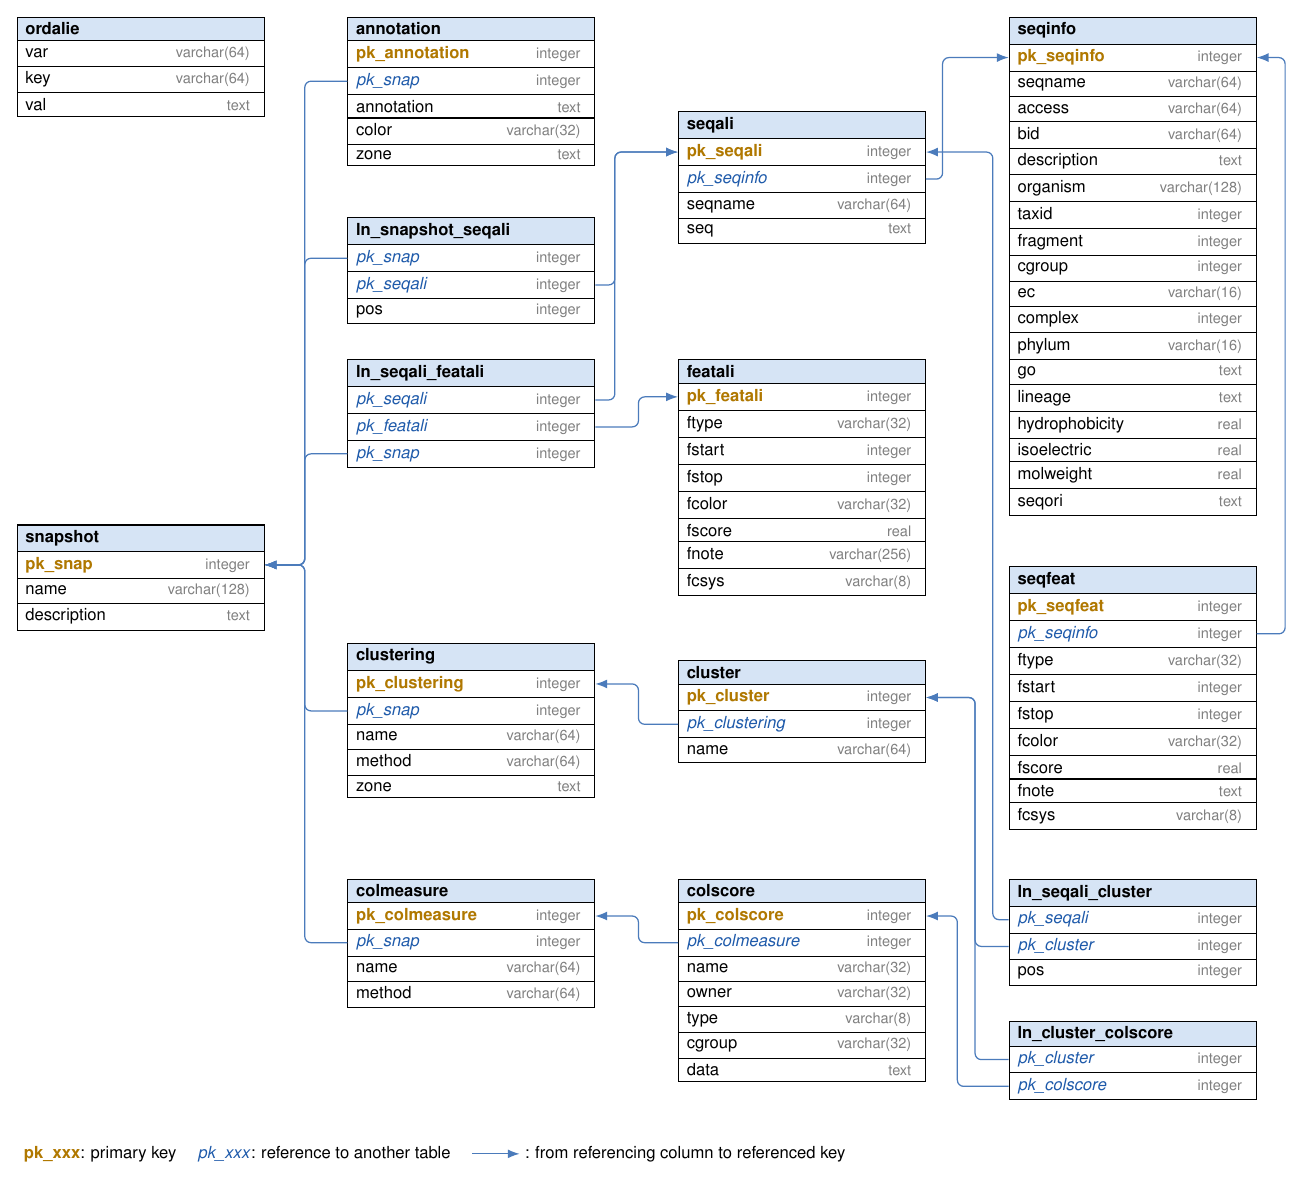
\includegraphics[width=\textwidth, keepaspectratio=true]{ordalie-db-scheme.png}
\caption{Scheme of the ordalie database.}
\label{ordalie-db-scheme}
\end{figure}

Ordalie takes advantage of this underlying database to store instances of alignments and their associated features.
In figure \ref{ordalie-db-scheme}, primary keys are shown in bold orange and columns referring to another table in blue italics; each arrow goes from the referring column to the primary key it refers to.
The "ordalie" table contains the session parameters (preferences, trees and overviews of all the instances) saved in the ORD file as (var, key, val) triplets, allowing the user to find the same state when the ORD file is re-opened.
The "seqinfo" table contains sequence information that is not linked to amino acid positions (accession, description, organism and taxonomy, EC number, GO terms, hydrophobicity, isoelectric point, molecular weight, ungapped sequence, ...).
The "seqfeat" table is used to store features data mapped onto the residue sequence of a "seqinfo" entry (type, start, stop, colour, score, note and coordinate system).
Upon loading of a new alignment file, Ordalie creates a first instance as being a read-only copy of this alignment stored as the "original alignment" in the "snapshot" table (instances are named snapshots in the database). This table contains all instances created so far along with their name and description.
The "seqali" table records the amino acid sequences, with their gaps, as they appear in the instances; each one refers to its "seqinfo" entry. A "seqali" entry is shared by all the instances in which the sequence is aligned the same way.
A link table "ln\_snapshot\_seqali" binds a given set of sequences to a given instance, together with their position in the alignment.
Accordingly, the "featali" table stores features attached to aligned sequences, in alignment coordinates. The link table "ln\_seqali\_featali" links a "featali" entry to a "seqali" entry within a given instance ("pk\_snap" column): since "seqali" entries are shared between instances, this is what keeps the features of each instance separate.
The "clustering" and "cluster" tables define a given clustering attached to an instance with its name, the \textbf{method and residue zones} used to compute it, and the resulting clusters with their names respectively. 
The set of sequences defining a given cluster, with their order, is available through the "ln\_seqali\_cluster" link table.
The "colmeasure" table corresponds to a conservation computation (column measurement) attached to an instance, with its name and the method used. The "colscore" table holds its results: for each score, its name, owner, type, conservation group and the values for each column of the alignment.
The conservation score for a given cluster is available through the link table "ln\_cluster\_colscore".
Finally, the "annotation" table contains the annotations the user adds to a given instance: text, colour and annotated zone (the zone refers to the sequences by their name, so that it does not depend on their order in the instance).
The "ordalie" table is not linked to any other table.
Structures are stored in separate databases (tables "pdb", "chains", "residues", "atoms" and "objetinit", the latter holding the 3D objects), not shown in figure \ref{ordalie-db-scheme}.
An ORD file (\texttt{.ord} extension) is a gzip-compressed tar archive of all these serialized databases.

\subsection{The FindPatterns syntax}
\label{findpatterns}
\attention{Ordalie implements a subset of the FindPatterns syntax: it is translated into a regular expression. Alternatives between parentheses must be single residues, a repeat count cannot exceed 255, and the \{\} and \{,n\} forms are not supported. \{n\} means exactly $n$ times.}

\subsubsection{Basic rules of syntax}
The search pattern can include any legal sequence character, and also include several non-sequence characters, which are used to specify 'OR' matching, 'NOT' matching, 'begin' and 'end' constraints, and repeat counts. For example, the pattern GASTE(X)\{20,30\}FTG means searching GASTE, followed by 20 to 30 of any amino acid, followed by FTG. Following is an explanation of the syntax for pattern specification.

\subsubsection{Implied Sets and Repeat Counts}
Parentheses () enclose one or more symbols that can be repeated a certain number of times. Braces \{\} enclose numbers indicating how many times the symbols within the preceding parentheses must be found.

If braces appear without preceding parentheses, the numbers in the braces define the number of repeats for the immediately preceding symbol. The second number may be missing. For example, the pattern GASG\{2,\}F means GAS, followed by at least 2 G, followed by F; GASG\{2\}F means GAS, followed by exactly 2 G, followed by F; GASG\{2,4\}F means GAS, followed by 2 to 4 G, followed by F. A repeat count cannot exceed 255. The letter X stands for any residue.

\subsubsection{OR Matching}
Specifying several symbol choices can be easily done by enclosing the different choices between parentheses and separating the choices with commas. For example, RGF(Q,A)S means RGF followed by either Q or A followed by S. Each choice must be a single residue. The pattern GAT(T,G)\{1,4\}A means GAT followed by 1 to 4 residues, each being T or G, followed by A. The sequence GATTGGA matches this pattern. There can be several parentheses in a pattern, but parentheses cannot be nested.

\subsubsection{NOT Matching}
The pattern GC\textasciitilde{}CAT means GC, followed by any symbol except C, followed by AT. The pattern GC\textasciitilde{}(A,T)CC means GC, followed by any symbol except A or T, followed by CC.

\subsubsection{Begin and End Constraints}
The pattern <GACCAT can only be found if it occurs at the beginning of the sequence. Likewise, the pattern GACCAT> would only be found if it occurs at the end of the sequence. Only one < and one > are allowed. The search is case-insensitive, and gaps are ignored.

\subsection{The GroupSim scoring method}
\label{meth-groupsim}
This is the GroupSim+ConsWin method of Capra and Singh \cite{groupsim}, with the identity matrix, as in the reference program of the authors. Residues B, Z and X are read as D, Q and gap. The gap is the 21st symbol of the alphabet: two gaps are identical. At column $p$, for a group $g$ of $n_g$ residues (gaps included, non-standard residues excluded), $n_g(a)$ of type $a$:
\begin{equation}
W_g = \frac{\sum_a n_g(a)\,(n_g(a)-1)/2}{n_g(n_g-1)/2} \qquad (W_g = 0 \textrm{ if } n_g < 2), \qquad
B_{gh} = \frac{\sum_a n_g(a)\,n_h(a)}{n_g\,n_h}
\end{equation}
With $N$ groups and $f_p$ the fraction of residues of the groups that are gaps:
\begin{equation}
\mathrm{GroupSim}_p = (1-f_p)\left(\frac{1}{N}\sum_g W_g - \frac{2}{N(N-1)}\sum_{g<h} B_{gh}\right)
\end{equation}
Columns with more than 10\% gaps, or with a group having more than 30\% gaps, are not scored. The conservation $C_p$ of a scored column is the Jensen-Shannon divergence between its residue frequencies (pseudocount 0.001, no sequence weighting) and the BLOSUM62 background distribution, times its fraction of non-gaps. The window conservation $\bar{C}_p$ is the mean of $C_j$ over the scored columns $j \neq p$, $|j-p| \leq 3$ (0 if there is none), mapped to $[0,1]$ over the alignment. The final score is
\begin{equation}
S_p = \lambda\,\mathrm{GroupSim}_p + (1-\lambda)\,\bar{C}_p, \qquad \lambda = 0.7
\end{equation}
The parameters are set in the \texttt{Defauts} array (\texttt{GroupSimWindow} = 3, \texttt{GroupSimLambda} = 0.7, \texttt{GroupSimColGap} = 0.1, \texttt{GroupSimGrpGap} = 0.3, \texttt{GroupSimMinGroupSize} = 2, \texttt{GroupSimTop} = 0.05). The reference program gives no cutoff: the fraction \texttt{GroupSimTop} of the best scored columns is marked.

\subsection{The Vector Norm scoring method}
\label{meth-vectornorm}
This method is based on a vectorial representation of the 20 amino acids. This representation can be the same as the one used in the VRP representation, or can be for example, a volume/polarity couple. The score for a given column $k$ can be computed then by:

\begin{equation}
  S(k) = \frac{n_c}{n_t}\,
         \frac{\left\| \sum_{i=1}^{n_c} \vec{V_i} \right\|}
              {\sum_{i=1}^{n_c} \left\| \vec{V_i} \right\|}
\end{equation}

where $\vec{V_i}$ is the vector of the residue of sequence $i$, $n_c$ is the number of residues in the column and $n_t$ the total number of sequences. This score lies between 0 and 1.

\subsection{The Feature File Format}
\label{chap-featurefile}
It is possible to import features into Ordalie through a features file. It is also possible to add items to an existing feature, or to create completely new ones.

The feature file format looks like:

\begin{verbatim}
# This is an example of a feature file
# Lines starting with # are comments and can be inserted anywhere

# Declare the feature (PROPAGATE all|group is optional)
FEATURE MyFeat PROPAGATE group

# seq. name; coord. system; start; stop; color; score; note
Q65P3D; LOCAL; 23; 57; red; 0.0; first item
Q65P3D; GLOBAL; 212; 345; blue; 0.0; second one
FLK14Q; local; 123; 234; red; 0.0; one more

# Then go to another feature
FEATURE STRUCT
P12345; global; 2112; 2541; green; ; add one
\end{verbatim}

Rules:
\begin{itemize}
  \item A feature is declared by \texttt{FEATURE <name>}, optionally followed by \texttt{PROPAGATE all} or \texttt{PROPAGATE group}: each item is then copied to all sequences of the alignment, or of the group of its sequence.
  \item Each item has exactly 7 fields separated by semicolons. Spaces are ignored except in the note.
  \item The sequence name must be the name used in the alignment.
  \item The coordinate system is \texttt{local} (positions in the sequence without gaps; PDB residue numbers for PDB sequences) or \texttt{global} (alignment columns), case-insensitive. Positions start at 1.
  \item The colour is a colour name or a \texttt{\#RRGGBB} value. An empty score is set to 0.0.
  \item Incorrect lines are reported and discarded. Items already present are not duplicated.
\end{itemize}
To add items to an existing feature, the feature name must be exactly identical to the one already present in the alignment, as feature names are case-sensitive.

\subsection{The superposition algorithm}
\label{app-superposition}
Given two sets of atomic coordinates A and B, the following algorithm will try to minimize the RMS (Root Mean Squared) distance between A and B by moving B onto A. The algorithm can be separated in the following steps:
\begin{itemize}
\item Compute the centre of mass (CDM) of the two sets and translate B atoms by the vector joining B CDM to A,
\item Compute the 3 main inertia axis for the two sets, which correspond to the three eigen vectors of the Eigen decomposition of the whole atomic coordinates set,
\item By turn, minimize the weighted RMS by rotating around the Eulerian angle associated to the current axis.
\item Stops when converged, and issue superposition information.
\end{itemize}

The output of this algorithm provides along with the RMS, the orientation matrix, translation vector, and rotations between the two molecules in different forms.

\subsection{The command line options}
\label{chap-cmdline}
\begin{center}
\begin{tabular}{|l|l|p{0.5\textwidth}|}
\hline
\textbf{Option}&\textbf{Values}&\textbf{Description}\\
\hline
\hline
-convert & TFA|MSF|XML|ALN|ORD & Converts the alignment into the given format and exits. Use \texttt{-outfile} to name the output file.\\
-outfile & <file> & Name of the converted file; its extension is replaced by the output format.\\
-precompute & 0|1 & Precompute clustering and conservation for each PFAM domain (default 0).\\
-threshold & <x> & Conservation threshold for the Threshold method; x must be between 51 and 100 (default 80).\\
-batch & & Run Ordalie without windows and exit when finished.\\
-downloadpdb & 0|1 & Download (1, default) or not (0) the PDB structures.\\
-showss & 0|1 & Show secondary structures at start-up.\\
-group & <file.clu> & Read the sequence groups from a \texttt{.clu} file.\\
\hline
\end{tabular}
\end{center}

The alignment file, if given, must always be the first argument, e.g.\ \texttt{ordalie myali.xml -convert TFA -outfile myali.tfa}. \texttt{ordalie help} prints a short help.

\newpage
\bibliographystyle{bmc-mathphys}
\bibliography{soft,methods,msa,dbs}


\end{document}



